\chapter{Machine Learning for Unfolding}
\label{chap:ml-for-unfolding}
\section{The Emergence of Machine Learning in Particle Physics}
\subsection{A Paradigm Shift in Data Analysis}
The past decade has witnessed a remarkable transformation in how particle physicists analyse data, driven by the adoption and adaptation of machine learning (ML) techniques.
%
This revolution has been catalysed by the confluence of three factors: the growing volume and complexity of data from modern collider experiments, the substantial increase in available computing resources, and the rapid advancement of ML algorithms and frameworks.
%
The Large Hadron Collider (LHC) alone produces petabytes of data annually, with individual collisions generating thousands of particles across multiple detector subsystems, creating a rich, high dimensional dataset that traditional analysis methods struggle to fully exploit~\cite{EnvironmentalCERN}.
%
Particle physics presents unique analytical challenges that align particularly well with the strengths of modern machine learning approaches.
%
The field routinely deals with high--dimensional feature spaces, complex non--linear correlations between observables, rare signal processes buried within overwhelming backgrounds, and some of the largest scientific datasets in existence~\cite{DiMeglio2017SubmitterResearch}.
%
These characteristics create an ideal test bed for advanced ML techniques, which excel at discovering patterns in precisely such environments.
%

The relationship between particle physics and machine learning is not entirely new.
%
Neural networks were first applied to high energy physics problems in the late 1980s and 1990s~\cite{Teodorescu2008ArtificialPhysics}.
%
However, these early applications were limited by computational resources and algorithmic capabilities.
%
The contemporary renaissance began around 2012--2014, coinciding with the broader deep learning revolution across computer science~\cite{TerrenceJ.Sejnowski2018TheIntelligence}.
%
This timing allowed particle physicists to leverage developments in computer vision, reinforcement learning, and generative modelling, adapting these techniques to the unique requirements of high-energy physics.
\subsection{Evolution of ML Applications in HEP}
\subsubsection{Classification Tasks}
        \label{subsubsec:classification-tasks}
The first wave of modern ML applications in particle physics focused predominantly on classification tasks, particularly signal/background discrimination and particle identification.
%
These problems are naturally framed as binary or multi--class classification, making them accessible entry points for machine learning techniques.
%
Boosted decision trees initially dominated these applications, particularly in the analysis chains that led to the Higgs boson discovery~\cite{Chen2014HiggsTrees}.
%
However, deep neural networks quickly demonstrated superior performance by automatically discovering complex patterns in high--dimensional data, often outperforming carefully hand--crafted physics--inspired variables~\cite{Baldi2014SearchingLearning, Baldi2015EnhancedLearning, Baldi2021DeepScience}.
%
For example, neural networks trained on low--level detector information have been shown to match or exceed the performance of approaches using physics--motivated high--level features for tasks like quark--gluon discrimination~\cite{Lee2019Quark-GluonNetworks} and top quark tagging~\cite{Pearkes2017JetTagging}
%
The ATLAS and CMS experiments have now incorporated deep learning based taggers for identifying hadronically decaying W/Z bosons~\cite{Chen2020BoostedLearning}, top quarks~\cite{Sirunyan_2020}, and Higgs bosons~\cite{2023TransformerATLAS}, significantly enhancing their sensitivity to new physics.
%
While early applications leveraged convolutional neural networks to exploit spatial correlations in calorimeter deposits~\cite{deOliveira2016Jet-imagesEdition, Komiske2018DeepDiscrimination} and recurrent or graph neural networks to handle variable--length, unordered collections of particles~\cite{Shlomi2020GraphPhysics, Qu2020ParticleNet:Clouds}, transformer architectures and foundation models have emerged as the current state of the art for many classification tasks~\cite{Qu2022ParticleTagging, Mikuni2025SolvingModels, VanStroud2024TransformersPhysics}.
%
Transformers excel at modelling complex dependencies through self--attention mechanisms, naturally processing sets of particles by capturing relationships between a span of pairs of particles simultaneously~\cite{Vaswani2017AttentionNeed}.
%
The Particle Transformer (ParT) architecture~\cite{Qu2022ParticleTagging}, specifically designed for HEP applications, has demonstrated superior performance on jet classification tasks by incorporating physics-motivated constraints while leveraging the power of self-attention to identify relevant particle interactions and correlations~\cite{Wang2024InterpretingTagging}.

\subsubsection{Regression and Anomaly Detection}
        \label{subsubsec:regression-and-anomaly-detection}
As the field matured, ML applications expanded beyond classification to include regression tasks, such as energy calibration~\cite{Holmberg2023JetPipeline}, pileup mitigation~\cite{Komiske2018PileupPUMML}, and particle momentum reconstruction~\cite{Haake2019Machine-learning-basedCollisions}.
%
These applications require models to predict continuous quantities rather than discrete classes, introducing additional complexity but extending ML based methods to a larger class of problems.
%
Simultaneously, unsupervised and weakly--supervised learning techniques emerged as powerful tools for anomaly detection, identifying potential new physics without explicit models~\cite{Belis2024MachinePhysics}.
%
These methods include autoencoders that flag events with high reconstruction loss, density estimation techniques that identify low--probability regions of phase space, and weakly--supervised classifiers that can distinguish data mixtures without event--by--event labels.

\subsubsection{Generative Models}
Perhaps the most significant recent development in ML for HEP has been the adoption of generative models, which learn to produce samples from complex probability distributions.
%
This capability is particularly valuable in particle physics, where accurate simulation is crucial but computationally expensive.

Generative adversarial networks (GANs)~\cite{Goodfellow2014GenerativeNetworks}, variational autoencoders (VAEs)~\cite{Kingma2019AnAutoencoders}, and normalizing flows~\cite{Kobyzev2019NormalizingMethods} have all been successfully applied to particle physics problems.
%
These models can generate synthetic collision events\cite{Moodie2022OptimisingNetworks}, simulate detector responses\cite{Darulis2022MachineSimulations, Xu2023GenerativeFlow}, and model complex differential distributions,\cite{Butter2025GenerativeMapping} often accelerating these processes by orders of magnitude compared to traditional Monte Carlo techniques.

The development of these generative models opened new possibilities for addressing inverse problems in particle physics, including the unfolding problem at the centre of this dissertation.
%
By learning complex, high--dimensional probability distributions directly from data, these methods offer a natural framework for tackling unfolding without the limitations of binning.

\subsection{Machine Learning Approaches to Unfolding}

The application of machine learning to unfolding represents a particularly promising frontier.
%
Traditional unfolding methods face significant challenges when dealing with high--dimensional spaces, correlated variables, and complex detector effects.
%
Machine learning approaches offer several potential advantages compared to traditional statistical methods.

Neural networks excel at capturing patterns in high-dimensional spaces, helping to mitigate the curse of dimensionality that plagues binned methods.
%
While traditional approaches become computationally prohibitive beyond a few dimensions, ML-based methods can effectively unfold many variables simultaneously`~\cite{komiske_preserving_2021}.
%
This capability enables jointly unfolding multi--differential measurements that would be impractical with conventional techniques.

Many ML--based unfolding methods operate directly on continuous distributions, eliminating binning bias and the need to predetermine bin boundaries.
%
This approach preserves fine--grained information that might otherwise be lost through discretization, and it enables the extraction of arbitrary derived observables from the unfolded distribution~\cite{Shmakov2025FullDiffusion}.
%
Furthermore, the architecture and training procedure of neural networks provide natural regularization without requiring explicit constraints.
%
Rather than manually tuning regularization parameters as in traditional methods, ML approaches incorporate regularization through network depth, width, dropout rates, and early stopping~\cite{Girosi1995RegularizationArchitectures}.
%
This implicit regularization can adapt more naturally to the varying complexity across different regions of phase space.

Additionally, some ML methods can learn the complete detector--to--particle transformation in a single training procedure, avoiding the separate steps of response matrix estimation and inversion required by traditional approaches.
%
This integrated optimization may reduce the compounding of uncertainties that can occur when errors propagate through multiple discrete stages of conventional unfolding pipelines
%
Once trained, many ML models also enable rapid inference on new data without retraining.
%
This amortized approach is particularly valuable for unfolding tasks that need to be repeated with slight variations, such as systematic uncertainty studies or detector condition changes~\cite{Brehmer2020EffectiveLearning}

    \subsection{Early successes and current challenges}
        Machine learning approaches to unfolding, such as \textsc{OmniFold}, have demonstrated promising results on jet substructure measurements, showing improved performance in high dimensional spaces compared to traditional methods.
        %
        \textsc{OmniFold} has been successfully applied in experimental analyses at H1~\cite{collaboration_measurement_2022, collaboration_unbinned_2023, collaboration_machine_2024, Arratia2025TowardsEvents}, STAR~\cite{song_measurement_2023, pani_generalized_2024}, T2K~\cite{Huang2025MachineTechnique}, ATLAS~\cite{collaboration_simultaneous_2024, collaboration_measurement_2025}, CMS~\cite{collaboration_measurement_2025}, and LHCb~\cite{collaboration_multidifferential_2023}, validating its practical utility.
        %
        However, these methods also face significant challenges.
        %
        Unlike traditional techniques with decades of validation, ML--based unfolding is relatively new and requires careful validation to ensure physical consistency.
        %
        Key concerns include proper uncertainty quantification, interpretability of the results, sensitivity to the training data, and potential biases introduced by the neural network architecture or training process~\cite{mishra_uncertainty_2021}.
        %
        Additionally, the field is still developing consensus on best practices for hyperparameter selection, architecture design, and evaluation metrics specific to unbinned unfolding.
        %
        The balance between flexibility and stability remains an active area of research, with new approaches continuing to emerge.

        As machine learning continues to evolve, both within particle physics and in the broader scientific community, we can expect further innovations in unfolding techniques.
        %
        Promising directions include physics--informed neural networks that incorporate known conservation laws or symmetries~\cite{raissi_physics-informed_2019}, uncertainty--aware models that provide more reliable error estimates~\cite{brehmer_guide_2018}, and techniques that combine the strengths of traditional and ML based approaches~\cite{willard_integrating_2022}.
        %
        The rapid progress in this field demonstrates the synergistic relationship between particle physics and machine learning.
        %
        Particle physics provides challenging problems and unique datasets that drive methodological innovations;
        %
        machine learning offers powerful tools that enable new measurements and insights.
        %
        This dissertation builds upon this foundation, exploring novel machine learning approaches to improve the precision and scope of differential cross--section measurements through novel unfolding techniques.

\section{Introduction to Neural Networks}
Neural networks are the fundamental building blocks of modern machine learning applications.
%
This section provides a rigorous mathematical framework for understanding neural networks, from their basic architecture to training methodologies.

    \subsection{Essential Concepts}
        \subsubsection{Neural Network Fundamentals}
            At its core, a neural network is a parametric function approximator loosely inspired by biological neural systems.
            %
            The fundamental unit, a neuron or node, computes a weighted sum of its inputs followed by a non-linear transformation:
            \begin{equation}
            y = \sigma(w^T x + b)
            \end{equation}
            where \(x \in \mathbb{R}^n\) is the input vector, \(y\in\R^{m}\) is the output vector, \(w \in \mathbb{R}^{n\times m}\) is a weight matrix, \(b \in \mathbb{R}^m\) is a bias term, and \(\sigma(\cdot)\) is a (typically non--linear) activation function.
            
            The \emph{depth} of a neuron is defined as the length of the longest path between the input and the neuron.
            %
            The set of all neurons at depth \(l\) is called \emph{layer} \(l\) of the network.
            %
            The width of a layer is the number of neurons in that layer.
            %
            This organization of neurons into layers, creates a hierarchical structure.
            %
            The \emph{depth}, \(d = l_{\max}\), of a neural network is defined as the depth of its deepest layer.
            %
            A graphical overview of these concepts is depicted in \cref{fig:nn-concepts}.
            \begin{figure}
                \centering
                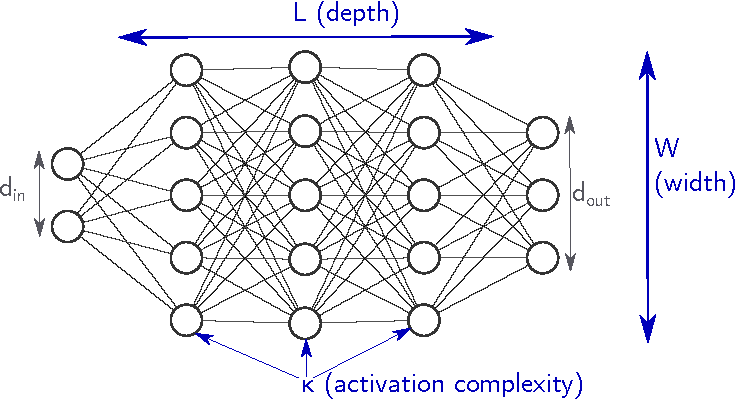
\includegraphics[width=\linewidth]{figures/chapter-03/CPWLNet_Descriptor.pdf}
                \caption[Neural network depth & width illustration]{Diagram illustrating the key structural parameters of a neural network: depth (number of layers), width (units per layer), and their relationship to input, hidden, and output layers~\cite{goujon_number_2023}.}
                \label{fig:nn-concepts}
            \end{figure}
            Any layer of a neural network except the input layer (often labelled layer \(0\)) and the output layer (\(l_{\max})\) is called a hidden layer.
            %
            A \emph{deep neural network} is a neural network with depth, \(d > 2\).
            %
            That is to say standard deep feed forward neural network consists of an input layer, \emph{more than one} hidden layers, and an output layer.%
            
            \cref{fig:shallow-nn} depicts a shallow neural network comprising a single hidden layer, while \cref{fig:deep-nn} shows a deep neural network with multiple hidden layers.
            %
            The shallow architecture can model only a limited set of simple, low level features, whereas the deep architecture composes successive non-linear transformations to extract increasingly abstract representations.
            %
            Increasing depth enhances representational capacity of the network and its capacity for hierarchical feature learning, albeit at the cost of greater computational complexity and potential optimization challenges.

            \newlength{\subfigheight}
            \setlength{\subfigheight}{4cm}
            \begin{figure}
              \centering
              \begin{subfigure}[b]{0.4\textwidth}
                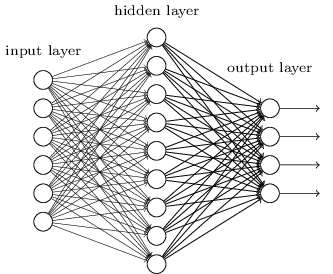
\includegraphics[height=\subfigheight,keepaspectratio]{figures/chapter-03/tikz35.png}
                \caption{Shallow network}
                \label{fig:shallow-nn}
              \end{subfigure}
              \begin{subfigure}[b]{0.5\textwidth}
                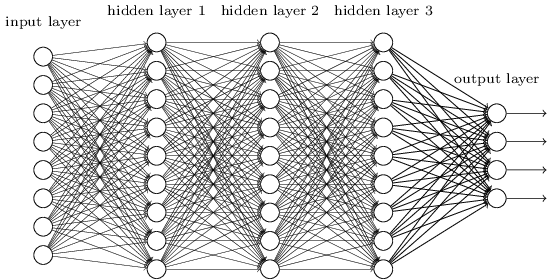
\includegraphics[height=\subfigheight,keepaspectratio]{figures/chapter-03/tikz36.png}
                \caption{Deep network}
                \label{fig:deep-nn}
              \end{subfigure}
              \caption[Shallow vs.\ deep NN]{Comparison between a shallow neural network (left) with a single hidden layer and a deep neural network (right) with multiple hidden layers~\cite{nielsen_neural_2015}.}
              \label{fig:shallow-deep}
            \end{figure}

            
            For a network with \(d\) layers, at each layer \(l\) the neural network computes
            \begin{equation}
                y^{(l)} = \sigma^{(l)}(W^{(l)} y^{(l-1)} + b^{(l)})
            \end{equation}
            where \(y^{(l)}\) represents the output of layer \(l, W^{(l)}\) is the weight matrix, \(b^{(l)}\) is the bias vector, and \(\sigma^{(l)}\) is the activation function of later \(l\).
            %
            By convention, \(y^{(0)} = x\) is the input, and \(y^{(d)} = y\) is the output.

            This architecture enables neural networks to approximate arbitrarily complex functions, as formalized in the Universal Approximation Theorem, which states that a deep neural network containing a finite number of neurons can approximate any continuous function on compact subsets of \(\mathbb{R}^n\) given certain mild conditions on the activation function.
            %
            Importantly, neural networks achieve superior approximation rates compared to traditional methods like polynomials, particularly in high dimensional settings.
            %
            While polynomial approximation suffers from the curse of dimensionality, requiring $\mathcal{O}(\varepsilon^{-d})$ parameters to achieve accuracy $\varepsilon$ in $d$ dimensions, neural networks can approximate smooth functions with rates of $\mathcal{O}(n^{-r/d})$ where $n$ is the number of parameters and $r$ is a smoothness parameter, often with significantly better constants and the ability to exploit compositional structure in the target function~\cite{petersen_optimal_2018,lu_expressive_2017}.

        
        \subsubsection{Forward propagation}
            The process of computing the network's output given an input is called forward propagation.
            %
            From its input \(y^{(0)} = x\) the network sequentially computes the output of each layer
            \begin{align}
                z^{(1)} &= W^{(1)}y^{(0)} + b^{(1)} \\
                y^{(1)} &= \sigma^{(1)}(z^{(1)}) \\
                &\nonumber \vdots \\
                z^{(d)} &= W^{(d)}y^{(d-1)} + b^{(d)} \\
                y^{(d)} &= \sigma^{(d)}(z^{(d)})
            \end{align}
            where \(z^{(l)}\) represents the pre--activation values at layer \(l\).
            %
            \cref{fig:forward-pass} depicts the computation in the forward pass.
            %
            Successive layer activations are computed by applying the weight matrices and bias vectors to the input, then passing the result through each layer's non-linear activation function until the final output is produced.
            \begin{figure}
                  \centering
                  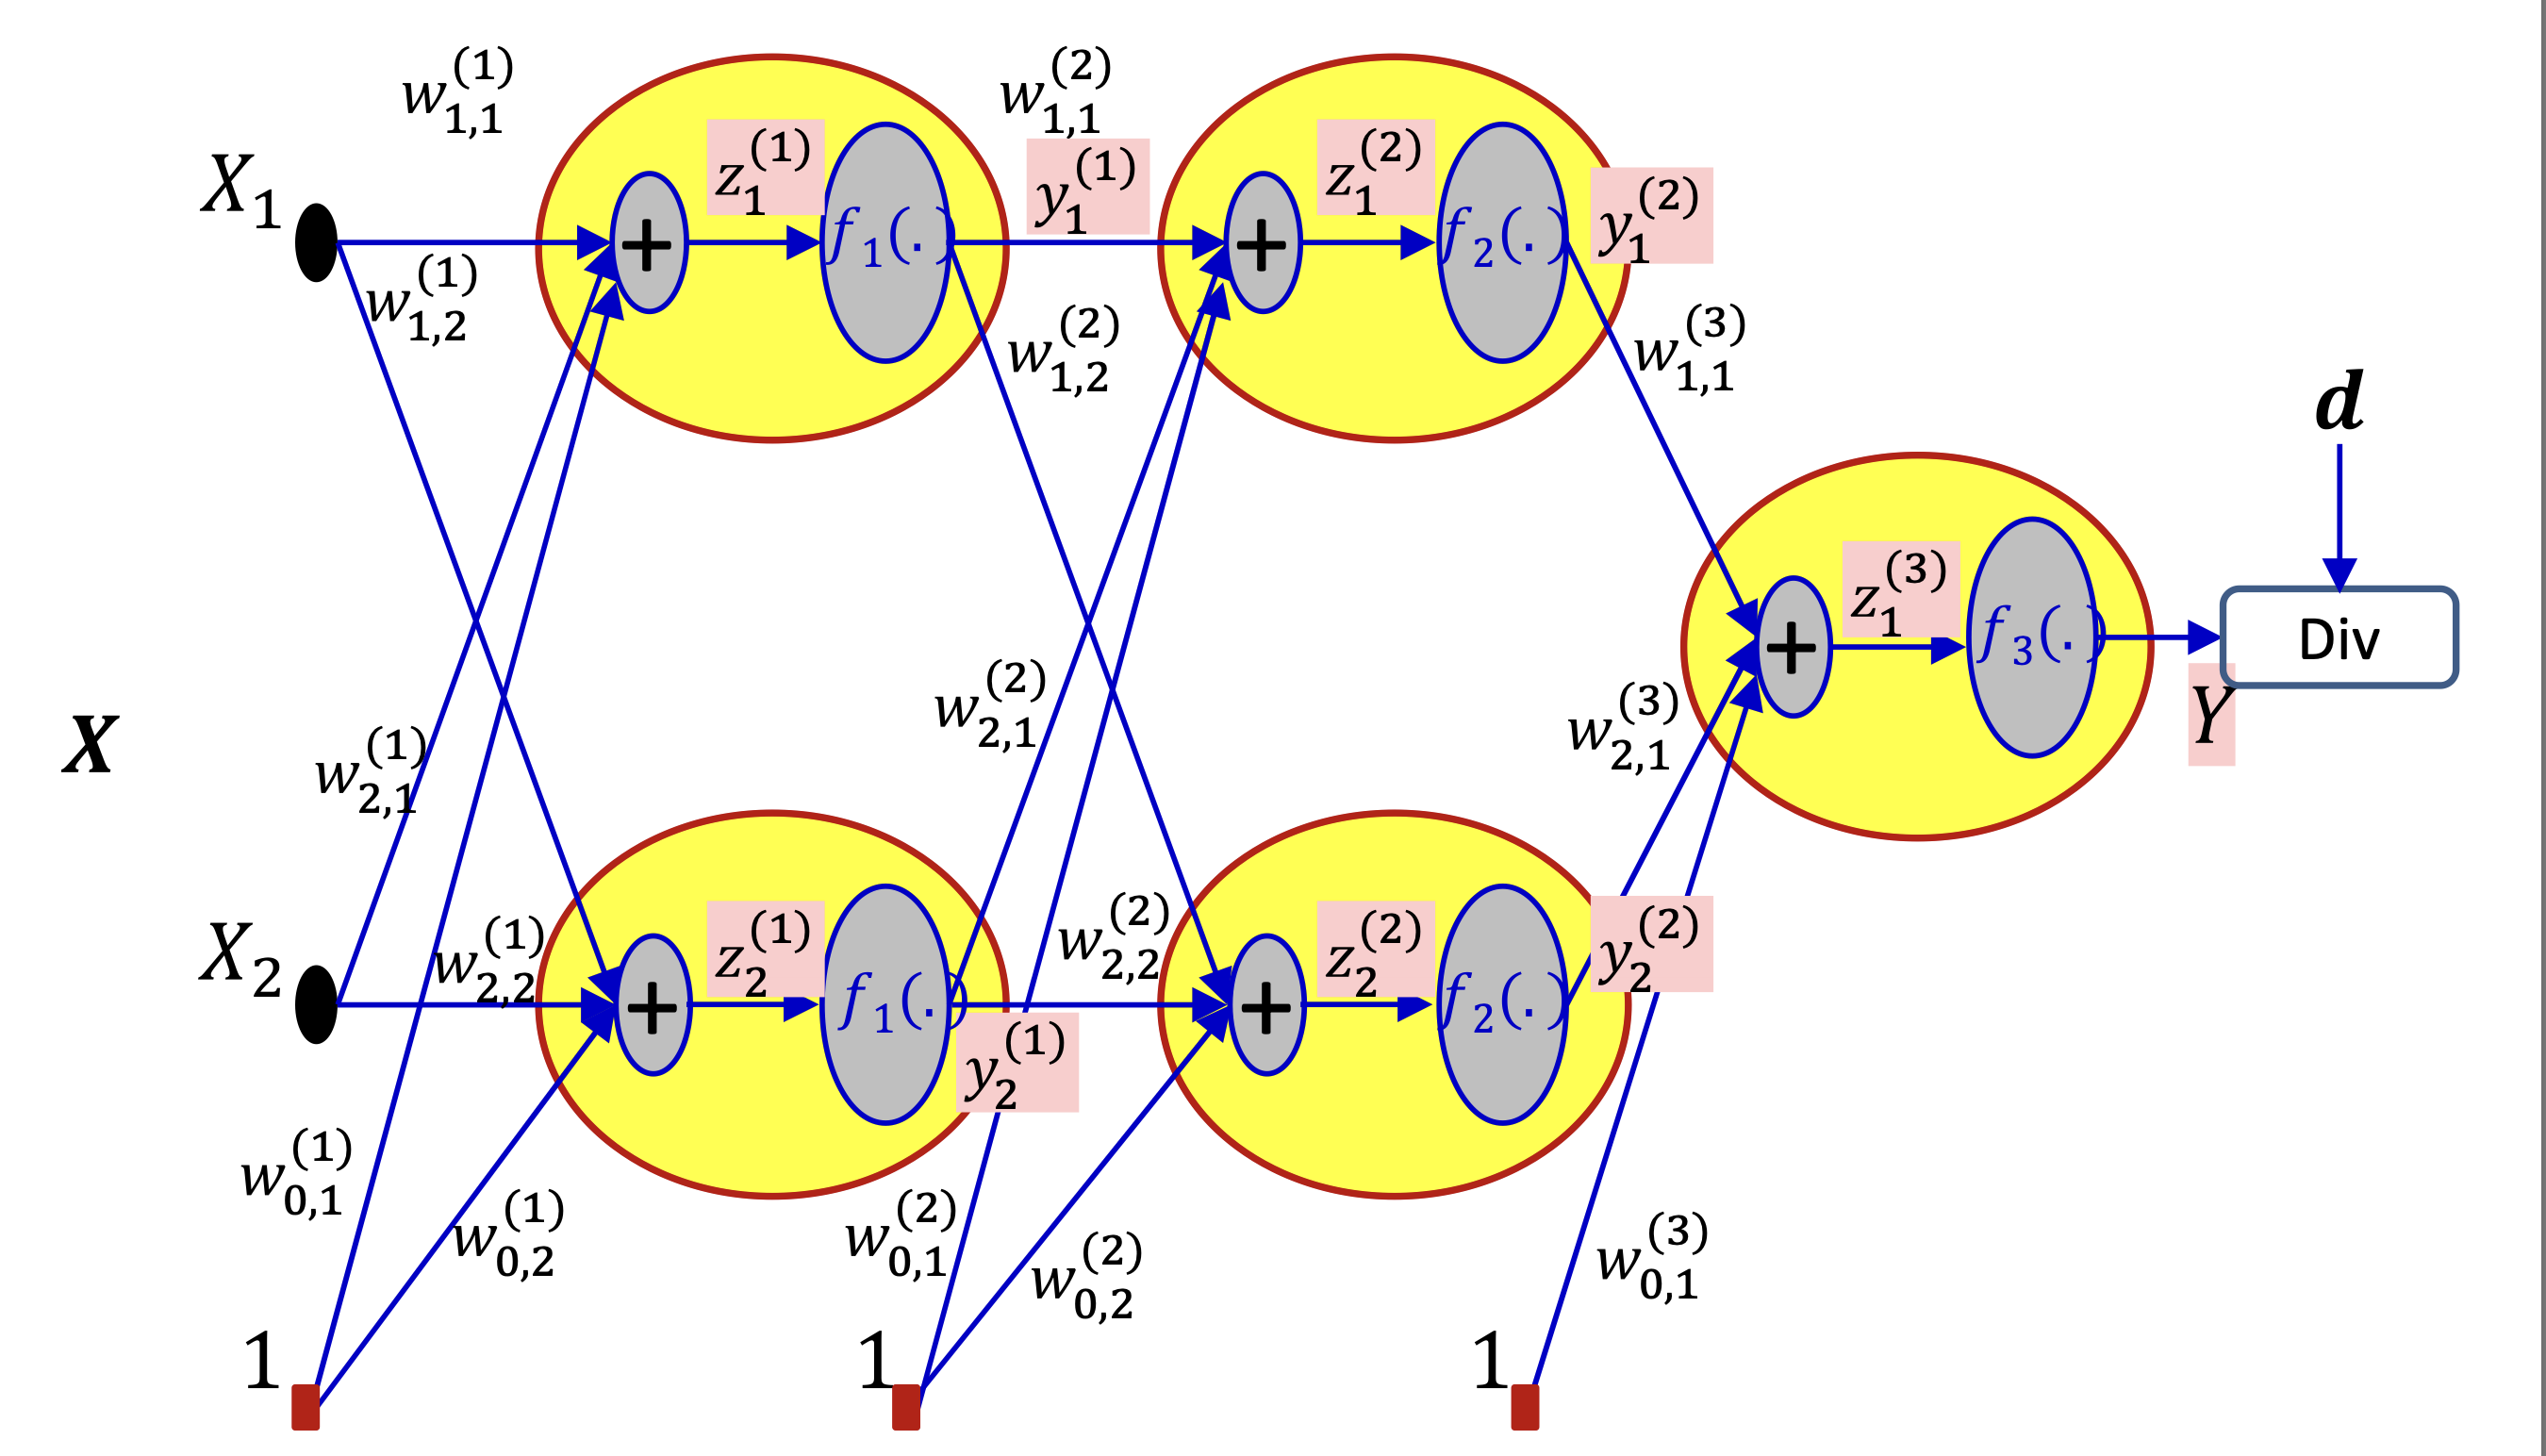
\includegraphics[width=0.8\textwidth]{figures/chapter-03/forwardpass.png}
                  \caption[Forward pass]{Illustration of the forward propagation process in a neural network, showing how the input vector is transformed by each layer's weights and biases and then passed through non-linear activation functions to yield the final output~\cite{noauthor_idl_nodate}.}
                  \label{fig:forward-pass}
            \end{figure}
        \subsubsection{Training objectives and loss functions}
            In order to quantify the accuracy with which a neural network \(f\) models a desired target function \(g\) for any particular input \(x\), a suitable measure of the error between \(f(x)\) and \(g(x)\) is required.
            %
            The \emph{divergence} \(\operatorname{Div}(x)\) is a continuous valued proxy for this error.
            %
            The goal of training can then be defined to be to learn the values of \(W\) that minimize the expected divergence.
            %
            (For notational convenience, from here on out, \(b\) will be collapsed into \(W\) as its \(0^{\textrm{th}}\) column;
            %
            the corresponding input, \(x_0 = 1\).)
            \begin{equation}
                \widehat{W} = \underset{W}{\arg\min}\int_X \operatorname{Div}\Big(f(x;\,W), g(x)\Big)\;p_X(x)\;\dd x
            \end{equation}

            In practice however, \(g\) is often not known for all \(x\in X,\) it is only known at some subset \(\qty{x_i}\subseteq X\).
            %
            The \emph{Loss function} \(\mathcal{L}\) is defined as the unbiased empirical average divergence between the neural network output and the target output over all training instances.
            \begin{equation}
                \mathcal{L}(W) = \frac{1}{N_X}\sum_{i=1}^{N_X}\operatorname{Div}\Big(f(x_i;\,W), g(x_i)\Big).
            \end{equation}
            The expected value of the loss function can be proved to be the expected divergence, which is precisely what it means for the loss function to be an unbiased estimate of the expected divergence.
            %
            However, this does not guarantee that minimizing the loss function will minimize the expected divergence.
        \subsubsection{Backpropagation and parameter learning}
            The training of neural networks revolves around finding the optimal values for weights and biases that minimize the loss function \(\mathcal{L}\)
            %
            Backpropagation is the algorithm used to efficiently compute gradients of the loss function with respect to each network parameter.
            %
            The core idea of backpropagation relies on the chain rule of calculus.
            %
            For a loss function \(\mathcal{L}\) and parameters \(\{W^{(l)}\}_{l=1}^d\) the network computes
            \begin{equation}
            \frac{\partial \mathcal{L}}{\partial W^{(l)}} = \frac{\partial \mathcal{L}}{\partial z^{(l)}} \frac{\partial z^{(l)}}{\partial W^{(l)}} = \delta^{(l)} (y^{(l-1)})^T 
            \end{equation}
            
            where \(\delta^{(l)} = \frac{\partial \mathcal{L}}{\partial z^{(l)}}\) is the error term for layer \(l\).
            %
            These error terms are computed recursively, starting from the output layer.
            \begin{align}
                \delta^{(L)} &= \frac{\partial \mathcal{L}}{\partial y^{(L)}} \odot \sigma'^{(L)}(z^{(L)}) \\
                \delta^{(l)} &= ((W^{(l+1)})^T \delta^{(l+1)}) \odot \sigma'^{(l)}(z^{(l)})
            \end{align}
            where \(\odot\) denotes the Hadamard (element-wise) product and \(\sigma'\) is the derivative of the activation function.
            %
            These derivatives are thus propagated backwards through the network, beginning at the output layer, propagated to the input layer.

        
        \subsubsection{Batching and Training Dynamics}
            In practice, neural networks are trained using mini--batch gradient descent, where parameter updates are performed using gradients computed on subsets (batches) of the training data. For a batch of size \(B\), the loss is
            \begin{equation}
                \mathcal{L}_{\text{batch}} = \frac{1}{B}\sum_{i=1}^B\mathcal{L}(x_i, y_i, W)
            \end{equation}
            Training proceeds in \emph{epochs}, where each epoch represents one complete pass through the training dataset.
            %
            To prevent overfitting, a separate validation dataset is typically used to monitor performance, and techniques such as early stopping may be applied when validation performance plateaus or degrades.
    \subsection{Neural Networks as Universal Approximators}
        The power of neural networks in physics applications stems from their ability to approximate arbitrary functions without requiring exponentially many parameters, unlike traditional methods such as polynomial approximation which suffer from the curse of dimensionality.
        %
        This property is formalized in the Universal Approximation Theorem, which has several variations but fundamentally states that feed-forward networks with a single hidden layer can approximate any continuous function on compact subsets of \(\mathbb{R}^n\) to arbitrary precision, given sufficient depth and width.
        \begin{theorem}[Universal Approximation Theorem]
        \begin{align}
            &\forall \sigma\in C^0(\R)\; \forall g\in C^0([0, 1]^n)\;\forall\epsilon > 0\;\exists M\in \R\\
            &\Bigg[\forall x\in\R\;|\sigma(x)| < M\implies \exists N\in\mathbb{N}\;\exists c, b\in \R^N\;\exists W\in \R^{N\times n}\\
            &\Big\{\forall z\in[0, 1]^n |c^T\sigma(Wz + b) - f(z)|<\epsilon\Big\} \lor \exists A\in\R\;\forall x\in\R\;\sigma(x) = A\Bigg].
            \end{align}
        \end{theorem}
        This theorem was first proved by Cybenko for sigmoid activation functions~\cite{cybenko_approximation_1989} and later extended by Hornik et. al to include a broader class of activation functions~\cite{hornik_multilayer_1989}. Modern versions of the theorem have relaxed various assumptions and expanded the results to deeper networks~\cite{augustine_survey_2024}.
        \subsubsection{Relevance to physics applications}
            The universal approximation property is particularly significant in physics.
            %
            Many physical systems are governed by complex, non-linear differential equations that lack closed-form solutions.
            %
            Neural networks can approximate these solutions without explicitly knowing the underlying equations, hence serving as excellent implicit simulators.
            %
            Additionally, physics problems often involve high dimensional spaces\footnote{e.g., the phase space for jet physics}.
            %
            Neural networks excel at learning in such spaces, where traditional numerical methods become computationally intractable.
            %
            The universal approximation property makes neural networks well--suited for these tasks, where the mappings to be learned are highly complex.

            When theoretical descriptions are incomplete, neural networks can discover patterns in data that suggest new physical models or refinements to existing ones.
            %
            Neural networks as universal approximators are also helpful for simulation based inference.
            %
            Modern physics often relies on computer simulations rather than closed--form likelihood functions.
            %
            Neural networks can approximate these implicit models for fast posterior inference.

            While the Universal Approximation Theorem guarantees the existence of a neural network capable of approximating any continuous function, it does not provide guidance on architecture design or training procedures.
            %
            Nor does the theorem provide any guarantees about the rate of convergence of training procedures.
            %
            In practice, deeper networks with multiple hidden layers have provide faster convergence, and greater parameter efficiency as discussed above.
            %
            However, the benefits of increasing depth are bounded, and decay exponentially, and hence the choice of architecture can involve carefully balancing the increased computational cost of a deeper network with the gains it provides.
            %
            Extensions of the theorem show that depth can exponentially reduce the number of neurons required to approximate certain function classes, explaining the empirical success of deep learning in physics applications.
            %
            These theoretical insights have motivated the development of specialized architectures tailored to specific physics problems, as will be discussed in subsequent sections.
    \subsection{Activation Functions, Optimization, and Regularization}
        \subsubsection{Activation Functions}
            Activation functions introduce non--linearity into neural networks, enabling them to learn complex patterns.
            %
            Several activation functions are commonly used in high energy physics applications.
            \begin{itemize}
                \item Sigmoid:
                    \[\sigma(z) = \frac{1}{1 + e^{-z}}\]
                    An activation function that outputs values between \(0\) and \(1\), it is most often used in problems involving binary classification.
                    %
                    The sigmoid activation function has a rich and important history as one of the earliest activation functions to be used in machine learning applications.
                    %
                    However, it suffers from vanishing gradient problems, where training instances far from its inflection point do not provide much information to the system.
                    %
                    Additionally, when many sigmoid functions are composed in deep networks, the resulting function can become very sharp and step--like, leading to training instabilities and poor gradient flow.

                \item Hyperbolic Tangent (tanh): \[\tanh(z) = \frac{e^z - e^{-z}}{e^z + e^{-z}}\]
                    The hyperbolic tangent function is very similar to sigmoid, except that it outputs values between \(-1\) and \(1\).
                    %
                    It is preferred in some applications because it is zero--centered, which can help in training dynamics, but it also suffers from the same vanishing gradient problems as the sigmoid.
                \item Rectified Linear Unit (ReLU): \[\text{ReLU}(z) = \max(0, z)\]
                    Simple, and incredibly computationally efficient, ReLU has become one of the most frequently used activation functions both within HEP and in the AI/ML space more broadly.
                    %
                    It addresses the vanishing gradient problem for positive inputs.
                    %
                    However, since it is simply zero for half its support, it can suffer from the ``dying ReLU" problem where units can become permanently inactive.
                \item Leaky ReLU: \[\text{LeakyReLU}(z) = \max(\alpha z, z)\]
                    \(\alpha\) is a small positive constant.
                    %
                    LeakyReLU is a modification of ReLU to allow small negative valued outputs~\cite{Maas2013RectifierModels}, which helps mitigate the dying ReLU problem.
                    %
                    Just a few of the many other variants that exist include Parametric ReLU (PReLU)~\cite{he_delving_2015} where \(\alpha\) is learnable, Exponential Linear Unit (ELU)~\cite{clevert_fast_2016} which provides smooth transitions for negative inputs, and Gaussian Error Linear Unit (GELU)~\cite{hendrycks_gaussian_2023} which has become popular in modern transformer architectures.

                \item Softmax: \[\text{softmax}(z_i) = \frac{e^{z_i}}{\sum_{j} e^{z_j}}\]
                        Softmax is most often used for multi--class classification output layers because it produces a probability distribution over classes.
                        %
                        The softmax reduces to the sigmoid when there only two classes, rendering binary classification simply a special case of multi--class classification.
            \end{itemize}
            These a but a few examples of the most common activation functions.
            %
            The choice of activation function significantly impacts network performance, convergence speed, and the occurrence of issues like vanishing or exploding gradients.
        \subsubsection{Optimization Techniques}
            As we discussed, neural network training is fundamentally an optimization problem.
            %
            Various algorithms have been developed to find optimal parameters efficiently.
            
            \paragraph{Gradient Descent}is the oldest and simplest approach to optimization.
            %
            It involves updating parameters in the direction of the negative gradient:
           \begin{equation}
                W_{t+1} = W_t - \eta \nabla_W \mathcal{L}(W_t)
           \end{equation}
            \(\eta\) is the learning rate.
            %
            While conceptually simple, gradient descent can be slow to converge and may get trapped in suboptimal solutions such as local minima.
            
            \paragraph{Stochastic Gradient Descent (SGD)}is an adaptation of gradient descent that updates parameters using gradients computed on mini--batches, introducing noise that can help escape local minima.
            \begin{equation}
            W_{t+1} = W_t - \eta \nabla_W \mathcal{L}_{\text{batch}}(W_t)
            \end{equation}
            \paragraph{Momentum based methods}accelerate convergence by accumulating a ``velocity" vector in directions of persistent reduction in the loss function.
               \begin{align}
                   v_{t+1} &= \gamma v_t + \eta \nabla_W \mathcal{L}(W_t) \\
                   W_{t+1} &= W_t - v_{t+1}
               \end{align}
               where \(\gamma\) is the momentum coefficient.
               %
               In HEP applications, a typical value of \(\gamma\) is \(0.9\).
            
            \paragraph{Adaptive Methods}are methods that vary the learning rate \(\eta\) over the course of the training rather than keeping it constant, and allow different learning rates for different dimensions of the input, rather than the traditional scalar learning rate that was constant across dimensions.
                \subparagraph{AdaGrad}
                    One of the earliest adaptive methods proposed was AdaGrad~\cite{duchi_adaptive_nodate}, which adapts learning rates per-parameter based on historical gradients.
                    %
                    AdaGrad was however limited by its aggressive learning rate reduction that slowed down training considerably.
                \subparagraph{RMSProp}
                    AdaGrad was soon replaced in almost all applications by RMSProp~\cite{hinton_neural_nodate}, an unpublished algorithm proposed by Hinton in course lectures~\cite{ruder_overview_2017}, which addresses AdaGrad's aggressive learning rate reduction.
                    %
                    Today, RMSProp is a widely used optimizer in ML applications, and is especially effective at stabilizing training when gradients are sparse and/or the loss function is dominated by saddle points.
            
            \paragraph{Adam}combines momentum based methods and RMSProp, and is currently the most widely used optimizer in ML applications~\cite{kingma_adam_2017}.
            %
                Adam's optimization procedure is can be described as
                 \begin{align}
                     m_t &= \beta_1 m_{t-1} + (1 - \beta_1) \nabla_W \mathcal{L}(W_t) \\
                     v_t &= \beta_2 v_{t-1} + (1 - \beta_2) (\nabla_W\mathcal{L}(W_t))^2 \\
                     \hat{m}_t &= \frac{m_t}{1 - \beta_1^t} \\
                     \hat{v}_t &= \frac{v_t}{1 - \beta_2^t} \\
                     W_{t+1} &= W_t - \frac{\eta}{\sqrt{\hat{v}_t} + \epsilon} \hat{m}_t
                 \end{align}
                Typical values in HEP applications are \(\beta_1 = 0.9, \beta_2 = 0.999, \epsilon = 10^{-8}\).
            
            
            
            \paragraph{Learning Rate Scheduling}is the process of dynamically adjusting the learning rate during training.
                %
                Some of the more common variants are step decay (reducing learning rate by a fixed factor after a set number of epochs), exponential decay (\(\eta_t = \eta_0 e^{-kt}\), and cosine annealing(\(\eta_t = \eta_{\min} + \frac{1}{2}(\eta_{\max} - \eta_{\min})(1 + \cos(\frac{t\pi}{T}))\)).
        \subsubsection{Regularisation Techniques}
            To improve stabilize the training, prevent overfitting, and increase generalization, various regularization methods are employed.

            \paragraph{\(L^p\) Regularisation} involves adding penalty terms to the loss function to penalize large weights.
                \begin{equation}
                    \mathcal{L}_{\textrm{reg}} = \mathcal{L} + \lambda_p\;\norm{W}^p.
                \end{equation}
                The most common values of $p$ are $1$ and $2.$
                %
                For certain applications, a hybrid $L1-L2$ regularisation may also be appropriate~\cite{shah_inverse_2016}.
            \paragraph{Dropout}is a form of regularization that involves randomly setting a fraction of neuron outputs to zero during training:
               \begin{equation}
                    y^{(l)}_{\text{dropout}} = m \odot y^{(l)}
               \end{equation}
               where \(m\) is a binary mask with entries drawn from a Bernoulli distribution with parameter $p\in [0, 1)$

            \paragraph{Batch Normalization} is the process of normalizing the inputs of a layer to have zero mean and unit variance.
                   \begin{align}
                   \hat{y}^{(l)} &= \frac{y^{(l)} - \mu_B}{\sqrt{\sigma_B^2 + \epsilon}} \\
                   z_{\text{BN}}^{(l+1)} &= W^T \hat{y}^{(l)} + b
                   \end{align}
                   where \(\mu_B\) and \(\sigma_B^2\) are the batch mean and variance.


        These regularization techniques, combined with appropriate optimization strategies and activation functions, form the foundation for effectively training neural networks for high energy physics applications.
        %
        The principles outlined here will be applied in subsequent sections focusing on specific neural network architectures and their applications to unfolding problems.
\section{Supervised Learning Approaches for Unfolding}
    Supervised learning provides a powerful framework for addressing the unfolding problem in particle physics. 
    %
    Unlike traditional matrix inversion methods, supervised learning approaches can leverage the flexibility and expressiveness of machine learning models to handle high-dimensional data and complex detector responses without requiring explicit binning schemes.
    \subsection{Mathematical Framework}
        Before exploring specific applications to unfolding, it is essential to establish what supervised learning is from a mathematical and statistical perspective.
        %
        Supervised learning represents one of the primary paradigms in machine learning where an algorithm learns a mapping from inputs to outputs using labeled training data.
        %
        Supervised learning involves using a dataset, \({D} = \{(x_1, y_1), (x_2, y_2), \ldots, (x_n, y_n)\}\) consisting of \(n\) input--output pairs.
        %
        Each input \(x_i \in {X}\) is a feature vector, and each output \(y_i \in {Y}\) is a label or target value.
        %
        The objective is to learn a function \(f: {X} \rightarrow {Y}\) that approximates the true relationship between inputs and outputs.
    
        Supervised learning searches over a space of functions \(f_\theta\)parameterized by \(\theta\) that minimizes the expected risk,
        %
        \begin{equation}{R}(f_\theta) = \mathbb{E}_{(x,y) \sim P(X,Y)}[\operatorname{Div}(y, f_\theta(x))]
        \end{equation}
        %
        where \(\operatorname{Div}\) is the divergence between the predicted output \(f_\theta(x)\) and the true output \(y\) y, and \(P(X,Y)\) is the joint probability distribution of inputs and outputs.
        %
        Since the true distribution \(P(X,Y)\) is unknown, we typically minimize the empirical risk
        %
        \begin{equation}
        \hat{{R}}(f_\theta) = \frac{1}{n}\sum_{i=1}^{n}\mathcal{L}(y_i, f_\theta(x_i))
        \end{equation}
        %
        Where \(\mathcal{L}\) is the loss function, the empirical expected divergence.
        %
        This empirical risk minimization is accomplished through the optimization of the loss functions described in the previous section using techniques like stochastic gradient descent and backpropagation.
    \subsection{Statistical Interpretation}
    \label{subsec:supervised_learning.statistical_interpretation}
        From a statistical standpoint, supervised learning can be viewed as conditional density estimation.
        %
        For classification problems, we estimate \(P(Y|X)\), the probability of a particular class given the input features.
        %
        For regression problems, we estimate the conditional expectation \(\mathbb{E}[Y|X]\) or the full conditional distribution \(P(Y|X)\).

        The choice of divergence function directly relates to the statistical assumptions being made.
        %
        The mean squared error, \[\operatorname{Div}(x) = (y - f_\theta(x))^2,\] corresponds to maximum likelihood estimation under Gaussian noise assumptions. The cross--entropy,
        \[
            \label{eq:bce}
            \operatorname{Div}(x) = -y\,\log f_\theta(x) - (1-y)\,\log(1 - f_\theta(x))
        \] corresponds to maximum likelihood estimation for categorical distributions.
        %
        Quantile divergences correspond to estimating specific quantiles of the conditional distribution

    \subsection{Types of Supervised Learning}
        Supervised learning problems broadly fall into two categories:
        \begin{enumerate}
            \item \textbf{Classification}:
            %
            When the output space \({Y}\) is discrete (categorical), the task is to predict the class label of a given input.
            %
            Common loss functions include cross--entropy and hinge loss.
            \item \textbf{Regression}:
            %
            When the output space \({Y}\) is continuous, the task is to predict a real--valued output.
            %
            Common loss functions include mean squared error, mean absolute error, and Huber loss.
        \end{enumerate}
        For unfolding problems, both paradigms can be relevant.
        %
        Classification approaches often estimate density ratios between distributions, while regression approaches directly estimate mappings between detector--level and particle--level observables.
    \subsection{Learning and Generalization}
        A fundamental aspect of supervised learning is generalization i.e. the ability of the model to perform well on unseen data.
        %
        This requires balancing two competing concerns, underfitting, when the model is too simple to capture the underlying structure of the data, and overfitting, when the model captures noise in the training data rather than the underlying structure.
        %
        Regularization techniques help prevent overfitting by constraining the complexity of the model.
        %
        For unfolding problems, regularization is particularly important due to the ill--posed nature of the inverse problem, where small variations in the data can lead to large variations in the prediction.
    \subsection{Evaluation}
        Supervised learning models are typically evaluated by measuring their performance on a separate test set not used during training.
        %
        Common evaluation metrics include accuracy, precision, recall, F1--scores, and ROC curves for classification problems; mean squared error, mean absolute error, and R-squared for regression problems

        In the context of unfolding, additional evaluation criteria can include physical consistency, preservation of known symmetries, and robustness to statistical fluctuations.
        %
    \subsection{Unfolding as a Supervised Learning Problem}
        At its core, unfolding seeks to recover the mapping from detector--level distributions to particle--level truth distributions.
        %
        This can be naturally framed as a supervised learning task where the model learns from pairs of detector--level and particle--level data generated through simulation.
        %
        The supervised learning approach to unfolding typically uses paired data \((z, x)\), where \(z\) represents particle--level quantities and \(x\) represents detector--level observations.
        %
        The forward problem (detector simulation) maps \(z \mapsto x\) through some response function, while unfolding attempts to estimate the inverse mapping.

        \subsubsection{Classification--Based Approaches}
            A prominent class of supervised learning methods for unfolding uses binary classification as its foundation.
            %
            This approach leverages the ability of classifiers to estimate likelihood ratios between distributions.
            %
            Of this class, \textsc{OmniFold} is perhaps the most widely adopted classification--based unfolding method and has been applied to several experimental measurements.
            %
            It uses an iterative procedure inspired by Iterative Bayesian Unfolding (IBU), generalizing it to the unbinned case.

            First, a classifier is trained to distinguish detector--level data from detector--level simulation.
            %
            The classification outputs are used to reweight simulation events.
            %
            Then another classifier is trained at particle level to transfer these weights back to the particle--level simulation.
            %
            These steps are repeated for some fixed number of iterations.

            This approach is particularly powerful for handling high--dimensional phase spaces where traditional binned methods become impractical.
            %
            \textsc{OmniFold} effectively retains the full phase space information without requiring dimensionality reduction.
        \subsubsection{Regression based calibration}
        \label{subsubsec:regression_calibration}
            Calibration corrects individual detector‐-level observables $x_i$ on an event by event basis.
            %
            Unfolding, in contrast, tackles the ill‐posed inverse problem of inferring a \emph{distribution} $p(z)$ from a smeared detector-‐level distribution $p(x)$.
            %
            Regression models that remap \(X\) are therefore calibration tools rather than unfolding tools \textit{per se}; they do not, by themselves, invert the response matrix or recover $p(z)$.
            
            It is still worthwhile to mention these regression based methods because they can reduce the bias and variance of traditional unfolding by feeding better‐behaved inputs into response‐matrix construction, and because probabilistic regressors provide conditional densities conditional PDFs that can be integrated into likelihood-‐based or Bayesian unfolding frameworks.
            \paragraph{Deterministic regression}
                Early neural network approaches attempted to learn a deterministic function $f$ that predicts a point estimate.
                %
                Although simple, such models tend to underestimate uncertainties, leading to biased predictions when used naively.
            \paragraph{Probabilistic regression.}
                Modern methods replace point estimates with conditional density estimators that yield conditional probability density functions.
                %
                Mixture‐-Density Networks~\cite{burton_mixture_2021, chen_physics-guided_2022, kuleshov_calibrated_2025, prassa_bayesian_2025, peng_efficient_2025}, Gaussian‐Process
                regressors~\cite{iwata_meta-learning_2023}, and normalizing flows~\cite{du_unifying_2024, bellagente_go_2022}
                have each been explored for this purpose, providing a principled propagation
                of detector smearing into unfolding‐stage uncertainties.

            In practice, conditional density can be sampled to build an event wise response ensemble, or inserted as the likelihood term in Bayesian unfolding.
            %
            Nevertheless, the global inverse problem remains one must still correct for resolution\footnote{Efficiency and acceptance effects also need to be corrected for, but they are typically not encapsulated in the response matrix for unfolding.} regression alone cannot address.
    \subsection{Regularization Strategies}
        Supervised learning approaches to unfolding must address the inherently ill--posed nature of the inverse problem.
        %
        This requires effective regularization strategies to prevent the amplification of statistical fluctuations.

        Neural network architectures themselves provide implicit regularization.
        %
        The choice of network depth, width, activation functions, and training protocols significantly impacts the solution's smoothness properties.
        %
        Convolutional layers, for instance, can encode physical priors such as translational invariance, constraining the space of possible solutions.

        In iterative approaches like \textsc{OmniFold}, early stopping serves as a form of regularization.
        %
        By halting the iteration process before full convergence, the method prevents overfitting to statistical fluctuations in the data.

        Domain--specific physics knowledge can also be incorporated into the learning process through custom loss functions, model architectures, or constraints.
        %
        For example, conservation laws, symmetries, or known theoretical behaviours can be encoded to guide the supervised learning process toward physically plausible solutions.
    \subsection{Advantages and challenges}
        Supervised learning approaches to unfolding can operate directly on unbinned data, avoiding information loss and artifacts from binning.
        %
        They scale better to high--dimensional observables and can effectively capture complex non--linear detector responses.
        %
        Additionally, they provide flexible regularization through model architecture and training.

        However, supervised approaches also face challenges.
        %
        They require large amounts of paired simulated training data with accurate detector modelling, where both detector level and particle level information must be available for each event.
        %
        Unless designed carefully for interpretability, the black box nature of neural networks can obscure the physical interpretation of the results.
        %
        For unbinned unfolding methods, uncertainty quantification remains challenging, particularly in capturing the correlations between events when computing confidence intervals.
        %
        Finally, validating the unfolding performance requires careful cross--checks and closure tests.

        Despite these challenges, supervised learning approaches represent a significant advancement in unfolding methodology, enabling measurements that would be impractical with traditional binned techniques,  in high--dimensional phase spaces relevant to modern particle physics analyses.



\section{Deep Learning Architectures}
High energy physics (HEP) presents unique data analysis challenges that have inspired the adoption and adaptation of specialized deep learning architectures.
%
These architectures are designed to handle the distinctive properties of particle physics data, including high dimensionality, sparsity, permutation invariance, and complex correlations.
%
This section explores the most prominent deep learning architectures employed in HEP applications, with particular emphasis on their relevance to unfolding tasks.
\subsection{Convolutional Neural Networks}
    Convolutional Neural Networks (CNNs) have found extensive application in HEP, particularly for analysing data with inherent spatial or geometric structure.
    %
    Originally developed for image recognition tasks, CNNs are well--suited for handling detector data that can be represented in image--like formats.
    
    A prominent application of CNNs in HEP is in the analysis of ``jet images" --- representations of energy deposits in calorimeters.
    %
    Treating jet constituents as ``pixels" in a coordinate system of pseudorapidity (\(\eta\)) and azimuthal angle (\(\phi\)) creates image--like representations that CNNs can process effectively.
    %
    For unfolding applications, CNNs can learn complex mappings between detector--level jet images and their corresponding particle--level representations.
    %
    The translation invariance property of CNNs naturally encodes physical symmetries, providing implicit regularization that is beneficial for the ill--posed unfolding problem~\cite{wu_dense_2021}.
    
    CNNs have also been successfully applied to model energy depositions in calorimeters~\cite{bhattacherjee_study_2019}.
    %
    These architectures can capture the spatial correlations in shower development patterns, enabling more accurate unfolding of particle energies and types from detector responses.
    %
    Three--dimensional CNNs have been employed to handle the full volumetric nature of calorimeter data, treating detector cells as voxels in a 3D space~\cite{yang_application_2024}.
    %
    These approaches have shown promising results in reconstructing particle properties from complex shower patterns~\cite{noauthor_deep_nodate, shi_pointrcnn_2019}.
\subsection{Recurrent Neural Networks}
    Recurrent Neural Networks (RNNs), particularly Long Short-Term Memory (LSTM) networks and Gated Recurrent Units (GRUs), have been applied to sequential aspects of HEP data analysis.
    %
    In many HEP applications, particles can be naturally ordered by properties such as transverse momentum or angular distance from a reference axis.
    %
    RNNs can process these ordered sequences while maintaining information about dependencies between particles.

    For unfolding tasks involving sequential data, RNNs can model the mapping between detector--level sequences and their particle--level counterparts, capturing complex ordered dependencies that might be lost in other architectures.
    %
    RNNs are also applicable to time--dependent detector responses or beam conditions that evolve over time.
    %
    By incorporating time information, these models could help unfold distributions that are affected by time--varying detector effects.
\subsection{Graph neural networks}
    Graph neural networks (GNNs) have emerged as one of the most promising architectural paradigms for HEP applications.
    %
    These networks explicitly model relationships between particles or detector elements as graphs, with nodes representing individual entities and edges representing their interactions or relationships.

    Particle interactions naturally form graph--like structures, where each particle can be considered a node with properties (features) such as momentum, energy, and charge.
    %
    GNNs can process these ``particle clouds" directly, without requiring conversion to image or sequence formats.
    %
    The key advantage of GNNs for unfolding is their ability to preserve the permutation invariance of particle collections;
    %
    the physical properties of a jet should not depend on the arbitrary order in which particles are processed.
    %
    By operating directly on graphs, GNNs respect this physical constraint.

    GNNs have also been applied to model the complex geometry of particle detectors, where detector elements can be represented as nodes and their physical or electronic connections as edges~\cite{Shlomi2020GraphPhysics, Thais2022GraphChallenges}.
    %
    This approach enables more accurate modelling of detector responses, which is crucial for reliable unfolding.
    %
    A specialized class of GNNs called Message Passing Neural Networks (MPNNs) show particular promise in physics applications.~\cite{Xu2024LearningTransformer}
    %
    These networks iteratively update node representations by passing information along edges, mimicking the way physical interactions propagate through a system.
\subsection{Transformer based architectures}
    Transformer architectures, which have revolutionized natural language processing, are increasingly being applied to HEP problems due to their ability to model complex dependencies through self--attention mechanisms~\cite{Spinner2024Lorentz-EquivariantPhysics}.
    %
    Transformers can naturally process sets of particles by using self--attention to capture relationships between all pairs of particles.
    %
    This makes them particularly well--suited for unfolding tasks involving collections of particles with complex inter--relationships.

    The Particle Transformer (ParT) architecture,\cite{Qu2022ParticleTagging} specifically designed for HEP applications, incorporates physics--motivated constraints and has demonstrated strong performance on jet classification tasks~\cite{Araz2025GraphLHC}.
    %
    Similar principles can be applied to develop transformer--based unfolding methods.
    %
    \textsc{OmniLearn}~\cite{Mikuni2025MethodTasks}, a foundation model built on the transformer architecture, demonstrates the ability of such models to improve the accuracy, precision, or speed of a wide range of physics tasks.\kd{Should I say all? It feels weird to catagorically say all, but maybe it really is all.}

    The attention mechanisms in transformers provide an additional benefit.
    %
    They can highlight which detector--level features are most informative for reconstructing particle--level properties.
    %
    This interpretability is valuable for understanding the unfolding process and identifying potential biases or limitations.
\subsection{Physics informed neural networks}
    A growing trend in HEP applications is the development of physics informed neural networks that explicitly incorporate domain knowledge about physical laws, conservation principles, and symmetries.
    %
    Networks that preserve known physical symmetries, such as Lorentz invariance or gauge symmetry, can provide more physically plausible unfolding results.
    %
    Architectures such as Lorentz Group Equivariant Networks\cite{Bogatskiy2020LorentzPhysics} ensure that the neural network respects these fundamental symmetries by design.
    %
    For problems where energy conservation is essential, specialized architectures can enforce this constraint by design.\kd{Re. ``Why would energy be conserved,"  for specific decay channels in hermetic detectors you would expect near-complete energy measurement, right? What I was trying to say was if your specific problem involves energy conservation, there are architectures that can enforce the constraint, not that all or even most problems have energy conservation. But maybe I'm misunderstanding, in which case, happy to remove this sentence.}
    %
    These networks ensure that the total energy is preserved between detector--level and particle--level representations, reducing the space of possible solutions and improving physical consistency.
    %
    Beyond specialized architectures, physical constraints can be incorporated into the loss function or network design.
    %
    For example, constraints on momentum conservation, charge conservation, or known physical boundaries of observables can guide the network toward physically plausible solutions.

    \subsubsection{Energy Flow Networks and Particle Flow Networks}
        Energy Flow Networks (EFNs) and Particle Flow Networks (PFNs)~\cite{Komiske2019EnergyJets} represent specialized deep learning architectures developed specifically for jet physics in HEP applications.
        %
        These networks leverage the fundamental principle that jets can be represented as collections of particles, each characterized by its energy or transverse momentum, and angular coordinates.

        The theoretical motivation for EFNs stems from the importance of infrared and collinear (IRC) safety in jet physics.
        %
        While traditional approaches like Energy Flow Polynomials~\cite{Komiske2018EnergySubstructure} provide a complete basis of handcrafted IRC--safe observables, EFNs offer a data--driven alternative that learns optimal IRC--safe representations directly from the energy flow of jets.
        %
        PFNs extend this framework by incorporating additional particle--level information beyond geometric coordinates, trading theoretical constraints for increased flexibility.
        
        Both architectures share a common structural feature that jet observables can be effectively decomposed into per--particle features and their aggregated relationships.
        %
        This decomposition naturally aligns with how QCD radiation patterns manifest in jet structure.
        %
        The networks implement this as follows:
        \begin{enumerate}
            \item \emph{Per--particle feature extraction:}
                Each particle is processed independently through a shared neural network, \(\Phi\), referred to the particle embedding network, mapping individual particle features to a latent representation.
            \item \emph{Permutation invariant aggregation:}
                The individual particle embeddings are combined through a permutation invariant operation.
                %
                For EFNs, this is specifically a weighted sum using particle energies, ensuring IRC safety.
                %
                PFNs typically use unweighted summation.
            \item \emph{Global processing:}
                The aggregated representation is processed by another neural network \(F\), called the latent space network to produce the final output.
        \end{enumerate}
        The distinction between these architectures is their treatment of IRC safety.
        %
        EFNs exclusively process geometric information \footnote{\((\eta,\phi)\) coordinates} with energy--weighted aggregation, ensuring that the learned representations respect IRC safety by construction.
        %
        This design choice guarantees that EFNs can only learn observables that are theoretically well--defined in QCD.
        %
        PFNs, conversely, can incorporate additional per--particle features such as particle type, charge, or identification probabilities.
        %
        While this makes PFNs more expressive for certain tasks, they do not provide IRC safety guarantees.
        
        For unfolding applications, this distinction has important implications.
        %
        EFNs' built-in IRC safety ensures that unfolded distributions preserve fundamental theoretical properties of QCD, providing implicit regularization aligned with physical principles.
        %
        This could eliminate certain unphysical solutions and help constrain the ill--posed nature of the unfolding problem.
        %
        PFNs offer complementary advantages when IRC--unsafe features, such as particle identification or flavour tagging information might be relevant, or even central, the unfolding task.
        
        Both architectures naturally handle the variable multiplicity of jets without requiring padding or truncation, making them well suited for realistic jet data.
        %
        In unfolding contexts, they can be employed as components within iterative approaches (like \textsc{OmniFold}).

        \paragraph{Relationship to other architectures}
            \subparagraph{Deep sets}
                From a broader machine learning perspective, EFNs represent specialized implementations of the Deep Sets~\cite{Sauer2023MeasurementCollider} paradigm for processing permutation invariant sets of varying sizes.
                %
                This connection to established theoretical frameworks facilitates both the analysis of these architectures and the development of future innovations in physics aware neural network design.
            \subparagraph{GNNs and transformers}
            \label{subpar:pfns-gnns-and-transformers}
                    PFNs can also be interpreted as a special case of more general architectures like Graph Neural Networks (GNNs) and transformers, which have gained prominence in particle physics applications.
                    %
                    In the GNN interpretation, a jet can be represented as a fully connected graph where particles are nodes and their relationships are edges.
                    %
                    While standard PFNs implicitly assume equal interactions between all particles through their summation pooling, GNNs explicitly model particle--particle interactions through message passing.
                    %
                    This allows GNNs to learn which particle relationships are most relevant for a given task, potentially capturing substructure patterns that simple summation might miss.
                    
                    The connection to transformers is even more direct.
                    %
                    The self--attention mechanism can be viewed as learning dynamic, data--dependent weights for particle interactions.
                    %
                    Recent architectures like the Particle Transformer~\cite{Qu2022ParticleTagging} and LorentzNet~\cite{GongAnTagging} use this idealearn complex inter--particle relationships while preserving desired invariances.
                    %
                    These transformer based approaches effectively interpolate between the simplicity of PFNs and the expressiveness of full graph networks, learning to focus on the most relevant particle combinations for each jet.
                    %
                    For unfolding applications, such architectures could potentially learn to identify and correct for detector--specific correlations between particles, though care must be taken to ensure the learned representations remain physically meaningful and do not overfit to detector artifacts.

The deep learning architectures discussed in this section provide a rich toolkit for addressing the challenges of unfolding in HEP.
%
By selecting and adapting architectures based on the specific properties of the data and the physics requirements of the analysis, researchers can develop more accurate and physically consistent unfolding methods.
%
The next section will explore advanced machine learning frameworks that build upon these architectures to provide even more powerful approaches to unfolding.

\section{Modern Machine Learning Frameworks}
This section explores sophisticated machine learning frameworks that have demonstrated significant potential for addressing the unfolding problem in high energy physics.
%
We examine three principal categories, generative models, discriminative models, and adversarial frameworks, each offering distinct approaches to learning complex distributions and relationships in particle physics data.
\subsection{Generative Models}
    Generative models represent a powerful class of machine learning techniques that aim to learn and characterize the underlying probability distribution of observed data.
    %
    Unlike discriminative models that focus on decision boundaries between classes, generative models capture the full data generation process, enabling them to produce new samples that resemble the training distribution~\cite{Kansal2023EvaluatingPhysics}.
    %
    The defining characteristic of these models is their ability to generate new, synthetic data points that follow the same statistical patterns as the training data.
    %
    This capability makes them particularly valuable for applications in particle physics where simulation of complex physical processes is essential~\cite{Carleo2019MachineSciences, Albergo2019Flow-basedSHANAHAN}.
    %
    In the context of unfolding, generative models offer a natural framework for modelling the mapping between particle--level and detector--level distributions.
    
    Generative models typically approach the learning task either by modelling the probability density function of the data explicitly, or by learning to generate samples from the target distribution without explicitly estimating the density.
    %
    Training generative models involves maximizing the likelihood of the data, though the specific approach depends on the model architecture.
    %
    For normalizing flows, for example, which have tractable likelihoods due to the change of variables formula, training directly maximizes the exact likelihood
    \begin{equation}
        \hat{\theta} = \underset{\theta}{\text{argmax}} \prod_{i=1}^{n} p(x_i | \theta)
    \end{equation}
    where \(p(x | \theta)\) is the conditional probability density function at \(x\) given \(\theta\) and \({x_i}_{i=1}^{n}\) are the training data.
    
    For Variational Autoencoders (VAEs)~\cite{Kingma2013Auto-EncodingBayes}, on the other hand, the true likelihood is intractable due to the latent variable integration.
    %
    Instead, VAEs maximize the Evidence Lower Bound (ELBO)~\cite{Kingma2019AnAutoencoders}, which provides a tractable lower bound on the log likelihood
    \begin{equation}
    \label{eq:ELBO}
        \log p(x) \geq \mathbb{E}_{q(z|x)}\qty(\log p(x|z)) - D_{\text{KL}}(q(z|x) || p(z))
    \end{equation}
    where the first term is the reconstruction loss and the second term is the KL divergence between the approximate posterior and the prior.
    %
    Both approaches ultimately aim to model the data distribution, but normalizing flows offer exact likelihood computation at the cost of architectural constraints, while VAEs trade exact likelihood for greater flexibility in model design.
    \subsubsection{Variational Autoencoders (VAEs)}
        Variational Autoencoders represent a class of deep generative models that combine the principles of variational inference with neural network based autoencoders~\cite{Bank2023Autoencoders}.
        %
        First introduced by Kingma and Welling in 2013~\cite{Kingma2013Auto-EncodingBayes}, VAEs provide a principled probabilistic framework for learning complex data distributions while enabling both generation of new samples and inference of latent representations.
        %
        Fundamentally, VAEs extend traditional autoencoders by imposing a probabilistic structure on the latent space.
        %
        While standard autoencoders learn deterministic encodings, VAEs encode inputs as probability distributions in the latent space.
        %
        This probabilistic approach enables principled sampling and uncertainty quantification, which are critical requirements for unfolding applications.

        The VAE architecture consists of two primary components, an encoder network \(q_{\phi}(z|x)\) which maps inputs \(x\) to a latent space distribution, typically parameterized as a multivariate Gaussian:
        \begin{equation}
        q_{\phi}(z|x) = \mathcal{N}(z|\mu_{\phi}(x), \text{diag}(\sigma^2_{\phi}(x)))
        \end{equation}
        where \(\mu_{\phi}(x)\) and \(\sigma^2_{\phi}(x)\) are parameters learned by the network, and a  decoder network \(p_{\theta}(x|z)\), which reconstructs inputs from latent samples, often parameterized as a Gaussian for continuous data,
        \begin{equation}
            p_{\theta}(x|z) = \mathcal{N}(x|\mu_{\theta}(z), \text{diag}(\sigma^2_{\theta}(z))),
        \end{equation}
        or a multivariate Bernoulli distribution~\cite{Fajtl2020LatentAutoencoder} for categorical data.

        This objective function minimized by VAEs, \cref{eq:ELBO}, balances two competing terms, the \emph{reconstruction term} \(\mathbb{E}_{q_{\phi}(z|x)}[\log p_{\theta}(x|z)]\) encourages accurate reconstruction, and the KL divergence term \(D_{KL}(q_{\phi}(z|x) \| p(z))\) that acts as a regulariser, encouraging the learned latent distribution to match a prior distribution.
        %
        The ELBO has deep connections to statistical mechanics and information theory.
        %
        The KL divergence term bears striking resemblance to the free energy minimization principle, where \(p(z)\) serves as an analogue to the ``ground state" or ``vacuum state" distribution~\cite{bilionis_free_2012}.

        Once trained, VAEs enable principled sampling by first sample from the prior distribution:\(z \sim p(z) = \mathcal{N}(0, 1)\), and then generating a new observation by passing \(z\) through the decoder: \(x \sim p_{\theta}(x|z)\)
        %
        This generative capability is particularly valuable for modelling the detector response in particle physics, where the mapping from particle--level to detector--level observables involves complex transformations and uncertainties.
        %
        Therefore in high energy physics, VAEs have found numerous applications including
        \begin{itemize}
            \item Fast detector simulation, where the VAE learns to map particle--level quantities to detector--level observables~\cite{Darulis2022MachineSimulations, hashemi_deep_2024},
            \item Anomaly detection for beyond Standard Model physics searches~\cite{liu_fast_2023},
            \item Dimensionality reduction of for processing collider data~\cite{yue_autoencoders_2024},
            \item Unfolding detector effects~\cite{erdmann_autoencoder-extended_2023}.
        \end{itemize}
        For unfolding applications specifically, several features of VAEs make them naturally suited for the task.
        %
        VAEs model the uncertainty in the inverse mapping from detector--level to particle--level distributions providing a direct probabilistic framework for downstream analysis.
        %
        One can regularise the problem by constraining the latent space to accord with the physics of the problem, which helps stabilize the training and reduce the variance.
        %
        Once trained, VAEs provide fast amortized inference, enabling efficient processing of large collision datasets

        Certain challenges posed by VAEs must be considered when selecting the appropriate model for a problem.
        %
        VAEs with Gaussian latent spaces can have limited expressivity because the latent space may be too restrictive for complex physical distributions.
        %
        Conversely, selecting a feature dense latent space (a) can deregularize the problem and (b) cause a loss of interpretability.
        %
        VAEs also tend to produce smoothed--out samples, potentially losing fine details in particle distributions.
        %
        Finally, balancing the reconstruction and KL terms requires careful tuning, and small changes in the hyperparameters can lead to significant changes in the learned function.

    \subsubsection{Normalising flows}
        Normalising flows represent a powerful class of generative models that learn the exact likelihood computation through a series of invertible, differentiable transformations.
        %
        Unlike VAEs, which approximate the likelihood, normalising flows directly learn a bijective mapping between the data distribution and a simple base distribution, typically a multivariate Gaussian.

        \paragraph{Mathematical formulation.}
            The core principle behind normalising flows is the change of variables formula from probability theory.
            %
            Given a random variable, \(Z\), with density \(p_Z(z)\) and an invertible, differentiable transformation \(f:\mathbb{R}^d \rightarrow \mathbb{R}^d\) the density of the transformed variable, \(x = f(z)\), is
            \begin{equation}
                p_X(x) = p_Z(f^{-1}(x)) \cdot \left|\det\left(\frac{\partial f^{-1}(x)}{\partial x}\right)\right|
            \end{equation}
            where \(\left|\det\left(\frac{\partial f^{-1}(x)}{\partial x}\right)\right|\) is the absolute value of the determinant of the Jacobian of \(f^{-1}\), which accounts for the change in volume elements due to the transformation.
            Normalising flows chain together multiple such transformations to create highly expressive mappings while maintaining invertibility.
            \begin{equation}
                f = f_K \circ f_{K-1} \circ \cdots \circ f_1
            \end{equation}
            The resulting density is
            \begin{equation}
                p_X(x) = p_Z(z) \cdot \prod_{k=1}^{K} \left|\det\left(\frac{\partial f_k^{-1}}{\partial f_{k-1}}\right)\right|
            \end{equation}
            where \(z = f^{-1}(x) = f_1^{-1} \circ \cdots \circ f_K^{-1}(x)\).

        \paragraph{Variations.}
            Since they were first proposed, several architectural innovations have expanded the expressivity and computational efficiency of normalizing flows.
            
            \subparagraph[Conditional normalising flows]{Conditional normalising flows.}
            \label{subpar:conditional-nfs}
                Conditional normalizing flows are a particularly promising variant for unfolding, where the transformation depends on additional conditioning variables~\cite{Winkler2019LearningFlows}.
                \begin{equation}
                    p_X(x|c) = p_Z(f^{-1}(x; c)) \cdot \left|\det\left(\frac{\partial f^{-1}(x; c)}{\partial x}\right)\right|
                \end{equation}
                In the unfolding context, the detector--level observables can serve as the conditioning variables, with the flow mapping from a base distribution to the particle--level distribution conditioned on detector measurements~\cite{Vischia2020NewUnfolding, Algren2023FlowReweighting}.
                %
                This approach enables explicit modelling of the posterior distribution
                (p(z | x)) that unfolding aims to estimate, even when the spaces have different dimensions, effectively learning the inverse detector response while accounting for the inherent ambiguities and information loss in the measurement process.
                %
                The conditioning mechanism preserves the exact likelihood computation that makes normalising flows so attractive for uncertainty quantification, while providing the flexibility needed to handle realistic experimental scenarios where dimensional consistency cannot be guaranteed.
                However, the choice of base distribution in normalising flows introduces an implicit prior that can significantly influence the unfolded results.
            \subparagraph{Other innovations.}
                Coupling layers, such as NICE~\cite{dinh_nice_2015} and RealNVP~\cite{dinh_density_2017}, partition the input dimensions and apply transformations to one part conditioned on the other, ensuring tractable Jacobian determinants
                \begin{gather}
                    y_{1} = x_{1} \\
                    y_{d+1} = x_{d+1} \odot \exp(s(x_{1})) + t(x_{1})
                \end{gather}
                where \(s\) and \(t\) are scale and translation networks.
    
                Autoregressive Flows, such as IAF~\cite{kingma_improving_2017} and MAF~\cite{papamakarios_masked_2018} model dependencies between dimensions through an autoregressive structure
                \begin{equation}
                    y_i = x_i \cdot \exp(s_i(x_{1})) + t_i(x_{1}).
                \end{equation}
                
                Continuous normalising flows~\cite{mathieu_riemannian_2020} formulate the transformation as an ordinary differential equation (ODE), offering increased flexibility.
        \paragraph{Applications.}
            Normalizing flows have gained significant traction in particle physics applications, including
            \begin{itemize}
                \item Simulation based inference: Using flows to perform likelihood--free inference for physics parameters~\cite{Green2020Gravitational-waveFlows},
                \item Fast detector simulation: Modelling the detector response through invertible mappings~\cite{krause_fast_2023},
                \item Phase space integration: Computing complex multidimensional integrals in perturbative calculations~\cite{Winterhalder2022TargetingNetworks},
                \item Unfolding detector effects~\cite{zeng_solving_2024}.
            \end{itemize}
            \subparagraph{Normalising flows for unfolding.}
                For unfolding specifically, normalising flows provide several compelling advantages.
                %
                The exact likelihood computation provided by the model enables principled uncertainty quantification in the unfolded distributions, allowing for rigorous statistical inference and error propagation.
                %
                The bijective nature of normalising flows aligns naturally with the physical process of detector effects and their inversion, as both involve transformations between probability distributions.
                %
                However, this direct correspondence is limited to cases where the measured and true distributions share the same dimensionality, a constraint that is frequently violated in realistic unfolding scenarios.
                In many experimental contexts, the detector and particle level quantities are not even the same physical quantity, so standard normalising flows, being bijective transformations, cannot directly handle these dimensional inconsistencies.
                
                Conditional normalising flows, discussed above in \cref{subpar:conditional-nfs}, elegantly address this limitation by treating the measured data as conditioning information rather than requiring a direct bijective mapping.
                %
                Capable of capturing complex distributions common in particle physics, both traditional normalising flows and different variants of flow--based models have been shown to be effective vehicles for unfolding, showing improved performance particularly for high dimensional and complex distributions~\cite{bellagente_go_2022}.

        \paragraph{Limitations.}
            Despite their theoretical elegance, normalising flows face several practical challenges in HEP applications.
            %
            Each version of the model makes different trade offs between expressivity, computational efficiency, and ease of training.
            %
            While normalising flows learn to transform from a simple base distribution (typically Gaussian) to the target distribution, this transformation is not unique---different choices of base distribution and flow architecture can lead to different learned mappings.
            %
            In unfolding applications, this prior dependence manifests as a form of regularisation bias, where the specific parametrisation of the flow influences which solutions are preferred among the many that could explain the observed data.
            %
            This issue becomes particularly acute in conjunction with the ill--posedness unfolding problems where multiple true distributions could have produced the same detector--level observations, making the implicit regularisation imposed by the flow architecture a critical but often unexamined aspect of the unfolding procedure.
            
            The invertibility requirement limits the types of transformations that can be used, and the computational cost of evaluating Jacobian determinants for high--dimensional data can impose practical limits on the dimensionality of the unfolding problem flow based methods can be applied to.
            %
            Furthermore, the prior dependence inherent in normalising flows presents a conceptual challenge for HEP applications.
            %
            The base distribution and architectural choices embed implicit assumptions about the structure of the solution space, potentially biasing the results in ways that are difficult to quantify or control.
            %
            Unlike some of unfolding methods that have been discussed so far, where regularisation assumptions are explicit and interpretable, the prior induced by the flow architecture operates through complex, high--dimensional transformations that resist straightforward interpretation.
            %
            This opacity complicates the assessment of systematic uncertainties and the comparison of results obtained with different flow architectures or base distributions.
            %
            Ongoing research continues to address these challenges through improved architectures and training procedures.
        
    
        \subsection{Discriminative Models}
            Discriminative models, introduced in \cref{subsubsec:classification-tasks,subsubsec:regression-and-anomaly-detection}, will be explored in greater depth in this section.
            %
            Discriminative models parametrise the conditional distribution, \(p(y|x)\) using a function \(f_\theta(x)\), where \(\theta\) represents the model parameters.
            \begin{equation}
                p(\,y\,|\,x\,) = p(\,y|\,f_\theta(\,x\,))
            \end{equation}
            For classification tasks with \(K\) classes, this typically takes the form of a categorical distribution,
            \begin{equation}
                p(\,y=k\,|\,x\,) = \frac{\exp f_\theta^k(x)}{\sum_{j=1}^K \exp f_\theta^j(x)}.
            \end{equation}
            The optimization objective is to maximize the conditional likelihood,
            \begin{equation}
                \mathcal{L}(\theta) = \prod_{i=1}^N p(\,y_i\,|x_i\,;\, \theta\,)
            \end{equation}
            or equivalently, minimizing the negative log--likelihood,
            \begin{equation}
                -\log \mathcal{L}(\theta) = -\sum_{i=1}^N \log p(\,y_i\,|\,x_i\,;\, \theta\,).
            \end{equation}
            This formulation provides a principled approach for both probabilistic classification and regression tasks that dominate HEP analyses.
        
            Modern discriminative models in particle physics typically employ neural networks with various architectures tailored to specific data structures.
            %
            The most common of these are fully connected networks, traditional deep neural networks with dense connections that transform inputs through a series of non-linear functions,
            \begin{equation}
                y_l = \sigma(W_l y_{l-1} + b_l)
            \end{equation}
            %
            Convolutional Neural Networks (CNNs) are useful for exploiting translational invariance in detector data through localized feature extraction.
            \begin{equation}
                y_{l,i,j}^k = \sigma\left(\sum_{m}\sum_{p,q} W_{p,q}^{k,m} y_{l-1,i+p,j+q}^m + b_l^k\right)
            \end{equation}
            where \(y_{l,i,j}^k\) represents the output of the \(k-\)th feature map at position \((i,j)\) in layer \(l\).
            %
            Recurrent Neural Networks (RNNs) are most often used to capture sequential information in particle trajectories.
            \begin{equation}
                y_t = \sigma(W_x x_t + W_y y_{t-1} + b)
            \end{equation}
            where \(y_t\) is the hidden state at step \(t\).
        
            \subsubsection{Training dynamics and optimization}
                Training discriminative models involves gradient--based optimization with regularization techniques to prevent overfitting.
                %
                The cross--entropy loss described in \cref{eq:bce}, derived from maximum likelihood is the most commonly used loss function to train discriminative models.
                %
                In some cases, specialized losses are like focal loss are used address class imbalances in rare physics processes.
                \begin{equation}
                    L_{\text{focal}} = -\sum_{i=1}^N (1-p_i)^\gamma \log(p_i)
                \end{equation}
                where \(p_i\) is the predicted probability of the correct class and \(\gamma\) is a focusing parameter.
    
            \subsubsection{Applications}
                Discriminative models serve multiple critical functions in particle physics analyses.
                \begin{itemize}
                    \item Event Classification: Separating signal from background events, with area under the ROC curve (AUC) values exceeding 0.99 in many recent LHC analyses,
                    \item Particle Identification: Distinguishing particle types based on detector signatures with significantly improved efficiency compared to cut--based methods,
                    \item Jet Tagging: Identifying jets originating from specific particles with significant performance gains over traditional approaches,
                    \item Unfolding: Estimating reweighting functions between detector-level and particle-level distributions, as implemented in \textsc{OmniFold}.
                \end{itemize}
                
                Despite their successes, the use of discriminative models can pose a series of challenges.
                %
                Neural network outputs often require calibration to provide accurate probability estimates for downstream statistical analysis.
                %
                These models are also typically considerably more complex than their generative counterparts, and may identify features that lack clear physical interpretation.
                %
                Quantifying model uncertainties remains challenging, particularly for ensemble approaches, when bootstrapping is computationally unfeasible.
                
                The following section examines a few specific discriminative model architectures that have proven effective in particle physics applications.
                %
                It begins with traditional approaches—--Support Vector Machines and Boosted Decision Trees--—which paved the way for ML adoption in HEP.
                %
                It then discusses modern deep learning architectures, graph neural networks and transformers, which have pushed the boundaries of what is achievable in physics analysis.
                %
                Each architecture offers unique advantages for different physics tasks, and understanding their relative strengths and limitations is crucial for selecting the appropriate model for a given analysis.\footnote{\begin{note}
                    {None of these architectures are used in the novel research presented in this thesis.
                    %
                    They are discussed here to provide a brief overview of historical and contemporaneous discriminative models used in the field.}
                \end{note}}
        \subsubsection{Traditional discriminative architectures}
            Before the deep learning revolution, particle physics relied heavily on classical learning methods that demonstrated remarkable effectiveness for classification and regression tasks.
            %
            These traditional discriminative architectures, while conceptually simpler than modern deep networks, established the foundation for machine learning adoption in high energy physics and continue to serve as reliable tools for many analyses.
            %
            Two methods in particular, support vector machines and boosted decision trees, have been used extensively in physics analysis due to their interpretability, robustness, and strong performance on the structured, tabular data typical of particle physics experiments.
        \paragraph{Support vector machines}
            SVMs find the maximum--margin hyperplane separating classes by solving the primary optimization problem
            \begin{gather}
                \min_{w,b} \frac{1}{2}\norm{w}^2 \\ \text{subject to } y_i\,(w^T x_i + b) \geq 1
            \end{gather}
            The dual formulation of this problem leads to the kernel trick, enabling non-linear decision boundaries:
            \begin{gather}
                \max_{\alpha} \sum_{i=1}^N \alpha_i - \frac{1}{2}\sum_{i=1}^N\sum_{j=1}^N \alpha_i\,\alpha_j \,y_i\, y_j \,K(x_i,x_j)\\\text{subject to }\alpha_i\ge0 \text{ and } \sum_{i=1}^N \alpha_i \, y_i = 0
            \end{gather}
            where\(K(x_i,x_j)\) is a kernel function.
        
            The choice of kernel dramatically affects SVM performance.
            %
            The most common choices in particle physics problems are the
            \begin{itemize}
                \item Linear kernel, \(K(x_i,x_j) = x_i^T x_j\), which is efficient for high--dimensional but linearly separable data,
                \item Radial basis function (RBF), \(K(x_i,x_j) = \exp(-\gamma\,\norm{x_i-x_j}^2)\), which is capable of capturing nonlinear detector responses, and
                \item Polynomial kernel \(K(x_i,x_j) = (x_i^T x_j + c)^d\), which models polynomial relationships in feature space.
            \end{itemize}
            
            SVMs have been applied across various particle physics processes.
            %
            Early applications in the Higgs discovery process demonstrated competitive performance and propelled these models forward in the discourse~\cite{bevan_support_2017}.
            %
            In analyses involving quark--gluon discrimination, SVMs with RBF kernels achieved discrimination power comparable to dedicated physics--inspired variables~\cite{sforza_support_2013, Anguita2004ModelClassifier}.
            %
            Attempts to construct SVMs for unfolding focus on their potential to estimate the density ratio between detector--level and particle--level distributions
            
            A persistent roadblock to their more widespread adoption has been the fact that traditional SVM implementations scale poorly with dataset size, \(\mathcal O(n^2)\) to \(\mathcal O(n^3)\).
            %
            Unlike deep networks, SVMs also require careful feature selection, and standard SVMs don't provide natural probability estimates, limiting their usefulness.
    
        \paragraph{Boosted decision trees.}
            Historically one of the most popular models employed in jet physics analyses, boosted decision trees (BDTs) combine weak learners \footnote{i.e. shallow decision trees} into a powerful ensemble.
            \begin{equation}
                F(x) = \sum_{m=1}^M \beta_m \,h_m(x)
            \end{equation}
            where \(h_m\) is the \(m-\)th tree and \(\beta_m\) is its corresponding weight.
            %
            Each tree recursively partitions the feature space according to information gain criteria,
            \begin{equation}
                \text{Gain} = \text{Impurity(parent)} - \sum_{j \in \{\text{children}\}} \frac{N_j}{N} \text{Impurity}(j)
            \end{equation}
            Several boosting algorithms have either been developed specifically for HEP or been employed in HEP analyses.
            \begin{itemize}
                \item \textbf{AdaBoost} iteratively reweights misclassified samples.
                \begin{equation}
                    w_i^{(t+1)} = w_i^{(t)} \cdot e^{\alpha_t \cdot \mathbf{1}(y_i \neq h_t(x_i))}
                \end{equation}
                where \(\alpha_t = \frac{1}{2}\ln\left(\frac{1-\epsilon_t}{\epsilon_t}\right)\) and \(\epsilon_t\) is the weighted error rate.
                \item \textbf{Gradient boosting} fits each tree to the negative gradient of the loss function with respect to the current prediction.
                \begin{equation}
                    h_m = \arg\min_h \sum_{i=1}^N L(y_i, F_{m-1}(x_i) + h(x_i))
                \end{equation}
                \item \textbf{XGBoost} incorporates second--order derivatives and regularization into the above schema.
                \begin{equation}
                    \mathcal{L}^{(t)} \approx \sum_{i=1}^n [g_i f_t(x_i) + \frac{1}{2} h_i f_t^2(x_i)] + \Omega(f_t)
                \end{equation}
            where \(g_i\) and \(h_i\) are the first and second derivatives of the loss.
            \end{itemize}
            
            BDTs have been extensively deployed in particle physics analyses.
            %
            The Toolkit for Multivariate Analysis (TVMA) integrated BDTs into the ROOT framework, cementing their place as a staple in HEP analyses.
            %
            BDTs were instrumental in the Higgs boson discovery by improving signal--to--background discrimination.
            %
            They can also be used in unfolding tasks, since they can model complex response matrices and estimate reweighting functions
            
            Despite their success, BDTs present several challenges, causing them to be eclipsed more recently by deep learning methods.
            %
            They struggle with highly correlated features common in detector data, and performance typically degrades in very high dimensional spaces.
            %
            Tree--based models also introduce discontinuities in the mapping function that can complicate uncertainty propagation.
        \subsubsection{Discriminative models and deep learning.}
            The transition from traditional learning to deep learning in particle physics has been driven by the need to handle increasingly complex data structures and extract more sophisticated feature representations.
            %
            While classical methods excel with engineered features and tabular data, deep learning architectures can automatically learn complex representations from raw or minimally processed data.
            %
            This capability has proven particularly valuable for particle physics applications involving complex topological relationships, variable length sequences, and high dimensional data.
            %
            Modern deep learning approaches have thus expanded the analytical toolkit available to physicists, enabling new insights that were previously difficult or impossible to obtain.
            \subsubsection{Graph Neural Networks}
                GNNs operate on graph--structured data, represented as \(G = (V, E)\)
                with nodes \(v_i \in V\) and edges \(e_{ij} \in E\).
                %
                The message--passing framework updates node representations through the rule
                \begin{equation}
                    y_i^{(l+1)} = \phi\left(y_i^{(l)}, \bigoplus_{j \in \mathcal{N}(i)} \psi(y_i^{(l)}, y_j^{(l)}, e_{ij})\right)
                \end{equation}
                where \(\phi, \psi\) are learnable functions, \(\mathcal{N}(i)\) denotes neighbours of node\(i\), and \(\bigoplus\) is the permutation--invariant aggregation operator.
        
                A few different specialized GNN variants have been developed with an eye towards specific physics applications.
                For example,
                %
                interaction networks model physical interactions between particles with explicit edge functions.
                %
                Dynamic graph CNNs construct graphs dynamically based on spatial proximity in detector space.
                %
                As discussed in \cref{subpar:pfns-gnns-and-transformers}, one possible interpretation of particle flow networks is as a special case of GNNs.
                %
                PFNs incorporate physics informed constraints into the message-passing mechanism.
                
                Similarly, HEP specific objectives functions have also been developed to train GNNs for HEP applications. 
                %
                These include node level classification for identifying individual particles,
                %
                graph level classification for categorizing entire events,
                %
                edge prediction for reconstructing particle interaction vertices,
                %
                and energy regression for estimating particle energies and momenta.
        
                Through these specialized architectures and objective functions, GNNs have shown remarkable performance across a range physics use cases.
                \begin{itemize}
                    \item Jet Tagging: Representing jets as graphs of constituents for improved identification performance
                    \item Event Reconstruction: Modeling entire collision events as interaction graphs
                    \item Tracking: Reconstructing particle trajectories from detector hits
                    \item Unfolding: Learning mappings between detector--level and particle--level observables while preserving physical symmetries
                \end{itemize}
                
                The most significant constraint on the use of GNNs in HEP is their computational complexity.
                %
                Message--passing operations scale with graph size and connectivity.
                %
                While their ability to naturally handle variable--sized inputs can be incredibly useful, implementing them requires careful batching strategies to maintain the differentiable structure of the network that backpropagation relies on.
    
        \paragraph{Transformer Models}
            Transformers process sequences through self--attention mechanisms,
            \begin{equation}
                \text{Attention}(Q, K, V) = \text{softmax}\left(\frac{Q\,K^T}{\sqrt{d_k}}\right)\,V
            \end{equation}
            where \(Q, K, V\) are query, key, and value matrices derived from input embeddings.
            %
            In HEP applications, self--attention enables modelling various relationships between particles, such as
            %
            permutation invariance for the natural handling of varying particle multiplicities,
            %
            long--range dependencies, for capturing correlations between distant detector regions,
            %
            and interpretable attention maps for visualizing learned physical interactions.
    
            Transformer models, which revolutionized the field of natural language processing, are increasingly being adopted for complex HEP tasks.
            %
            While transformers were originally designed to process sequential data where order not only matters, but also is expressly important to the learned representation, they can be adapted to be permutation invariant, a necessary property for particle physics applications where the ordering of particles or constituents is typically arbitrary and physically meaningless.
            %
            In jet classification tasks, transformers process jets as collections of constituents rather than sequences, learning representations that are invariant to the order in which particles are presented.
            %
            This permutation invariance is achieved through modifications to the standard transformer architecture, such as removing positional encodings or using specialized attention mechanisms that treat input particles symmetrically.
            %
            Transformers have been applied to event-level classification tasks in particle physics, with applications including jet classification and event categorization~\cite{Kheddar2025ImageSurvey, mikuni_point_2021, builtjes_attention_2025}.
            %
            This capability has proven particularly valuable for event level analysis, where the transformer can capture complex relationships between particles throughout the entire collision while respecting the fundamental symmetries of the underlying physics.
    
            However, despite their potential, some of the characteristics of transformer models have hindered their widespread adoption in HEP.
            %
            Self attention operations scale quadratically with sequence length, constraining the size of attention modules~\cite{Vaswani2017AttentionNeed}.
            %
            Transformer models typically require large training datasets~\cite{zhao_large-scale_2024}, as a consequence of which, training runs can rarely exceed one epoch~\cite{miao_locality-sensitive_2024}.
            %
            Hence, while transformers can learn surface level relationships extremely effectively, they are limited in their ability to learn deeper structure that would require multiple passes over each data point to discover~\cite{caron_trackformers_2025, Wang2024InterpretingTagging, stroud_transformers_2024}.
    
    \subsection{Adversarial models.}
        Adversarial models leverage the competitive dynamics between two neural networks to achieve powerful generative and discriminative capabilities.
        %
        These models have revolutionized high energy physics applications by enabling novel approaches to simulation, unfolding, and domain adaptation.
        %
        Fundamentally different from traditional architectures, adversarial models employ a game theoretic framework that can capture complex, high dimensional distributions and transformations relevant to particle physics.
    
        Adversarial models are typically constructed using two competing neural networks, a generator \(g\) and a discriminator \(d\).
        %
        The generator attempts to produce outputs that the discriminator cannot distinguish from real data, while the discriminator attempts to correctly classify inputs as either real or generated.
        %
        This minimax game is formalized as
        \begin{equation}
            \max_g \min_d L(d, g) = -\mathbb{E}_{x \sim p(x)}[\log d(x)] - \mathbb{E}_{z \sim q(z)}[\log\qty(1 - d(g(z)))]
        \end{equation}
        where \(p(x)\) is the true data distribution, \(q(z)\) is a latent space distribution\footnote{typically Gaussian noise, though in the variations presented in this thesis, \(q(z)\) will most often be the generation distribution.}, \(g(z)\) maps the latent space to the data space, and \(d(x)\) outputs the probability that
        \(x\) came from the real data rather than the generator.
    
        In the context of particle physics, this framework can be extended to incorporate domain specific constraints and physical laws, leading to specialized variants such as
        \begin{equation}
            \begin{split}
                \max_g \min_d L(d, g) &= -\mathbb{E}_{x \sim p_{\text{data}}(x)}[\log d(x)] \\
                &\quad - \mathbb{E}_{z \sim p_z(z)}[\log(1 - d(g(z)))] + \lambda \mathcal{R}(g)
            \end{split}
        \end{equation}
        where \(\mathcal{R}(g)\) represents physics--informed regularization terms that enforce conservation laws, symmetries, or other physical constraints, weighted by hyperparameter \(\lambda\).

        The following sections will discuss some of the most common variants of adversarial models, and how they can be applied to the HEP analyses.\footnote{\begin{note}{Not all architectures discussed in the following sections are used in the novel research presented in this thesis. They are included here to provide a more complete picture of the landscape of adversarial models relevant to particle physics. }\end{note}}
    
    \subsubsection{Generative Adversarial Networks (GANs)}
    \label{subsubsec:GANs}
        Generative Adversarial Networks (GANs) represent a fundamentally different approach to generative modelling, employing an adversarial training framework rather than explicit density estimation~\cite{UCLDeepMind}.
        %
        First introduced by Goodfellow et al. in 2014~\cite{Goodfellow2014GenerativeNetworks}, GANs have revolutionized generative modelling through their ability to produce remarkably realistic samples, particularly for high dimensional data like images~\cite{brock_large_2019, karras_analyzing_2020, karras_progressive_2018, zhang_self-attention_2019, karras_style-based_2019, denton_deep_2015}.
        %
        By training the two networks simultaneously in the aforementioned minimax game, the generator learns to produce increasingly realistic samples that can fool the discriminator, while the discriminator improves its ability to distinguish real from generated samples.
    
        From a theoretical perspective, the GAN objective can be interpreted as minimizing the Jensen--Shannon divergence, or a variant thereof, between the data distribution and the generator distribution~\cite{lin_divergence_1991, nielsen_jensenshannon_2019, manning_foundations_1999, endres_new_2003, Altheimer2012JetBenchmarks, fuglede_jensen-shannon_2004}.
        %
        Training proceeds by alternating between optimizing the two networks using opposing gradient information, \textit{viz.} \(d\) is updated using gradient descent,
        \begin{equation}
            \theta_d \leftarrow \theta_d - \eta \nabla_{\theta_d} L(d, g),
        \end{equation}
        and \(g\) is updated using gradient ascent,
        \begin{equation}
            \theta_g \leftarrow \theta_g + \eta \nabla_{\theta_g} L(d, g).
        \end{equation}
        
        In equilibrium, the generator produces samples indistinguishable from the real data distribution, and the discriminator outputs a probability of 0.5 for all inputs.
        %
        Formally the optimal discriminator computes
        \begin{equation}
            d(x) = \frac{p_{\text{data}}(x)}{p_{\text{data}}(x) + p_g(x)}\quad\text{for all } x
        \end{equation}
        and the optimal generator perfectly captures the data distribution
        \begin{equation}
            p_g(x) = p_{\text{data}}(x)
        \end{equation}
        
        In practice, reaching this optimum can be challenging due to the min--max nature of the objective, leading to training instabilities like mode collapse and oscillations.
        %
        For this reason numerous GAN variants have been proposed to address stability issues and enhance performance.
        
        In addition to architectural modifications, there also exist techniques such as spectral normalisation, which can be applied to GAN--like methods across the board to potentially improve stability.
        %
        \emph{Spectral normalisation}, whihc controls the Lipschitz constant of the discriminator by normalizing its weights,
        \begin{equation}
            W_{\text{SN}} = \frac{W}{\sigma(W)},
        \end{equation}
        where \(\sigma(W)\) is the spectral norm of weight matrix \(W\), provides additional tools to avoid training instabilities in GANs~\cite{Terjek2019AdversarialRegularization, miyato_spectral_2018}.
        %
        Spectral normalization, which has long been studied for its effectiveness in regularizing inverse problems~\cite{Clason2021RegularizationProblems, Engl2020RegularizationProblems, hansen_6_2006}, therefore is a natural fit for GAN based methods for unfolding.

        \paragraph{Applications}
            These advances have made GANs more practical for scientific applications like those in particle physics.
        
            In high-energy physics, GANs have found diverse applications.
            \begin{itemize}
                \item \textbf{Fast detector simulation:} GANs can approximate the mapping from particle-level to detector-level observables, significantly accelerating the simulation process~\cite{maevskiy_generative_2023, rogachev_gan_2023, Paganini2018CaloGANNetworks, bandieramonte_fastcalogan_2023, giannelli_caloshowergan_2024, khattak_fast_2022}
                \item \textbf{Event generation:} GANs can generate collision events, potentially replacing or augmenting traditional Monte Carlo approaches~\cite{butter_how_2019, di_sipio_dijetgan_2019}
                \item \textbf{Anomaly detection:} Identifying rare or anomalous collision events that deviate from Standard Model predictions~\cite{vaslin_gan-ae_2023, DiMattia2019ADetection, Belis2024MachinePhysics, Knapp2021AdversariallyQuark}
            \end{itemize}

            \subparagraph{GANs for unfolding.}
                The unfolding problem in high energy physics presents a two--level challenge that makes it particularly well suited for GAN based approaches.
                %
                At its core, unfolding seeks to recover the true particle level distribution from the measured detector level observations~\cite{noauthor_statistics_2010, FreiburgHEP, Segura2024APhysics, Berger2017LectureATLAS, blobel_unfolding_2002}. 
                %
                This inverse problem is complicated by the fact that detector measurements are affected by numerous physical processes including finite resolution, acceptance limitations, detector inefficiencies, and backgrounds~\cite{agostini_bayesian_2003, schmitt_tunfold_2012}.
                %
                The mapping from particle level to detector level involves complex non-linear transformations that traditional unfolding methods struggle to capture fully~\cite{hocker_svd_1996, adye_unfolding_2011}.
                
                GANs offer several fundamental advantages for addressing this two--level structure.
                %
                First, the adversarial training framework naturally accommodates the forward and inverse mappings between detector and particle levels without requiring explicit likelihood functions~\cite{datta_unfolding_2018, hashemi_deep_2024, bellagente_how_2020}.
                %
                The generator network learns to transform detector--level distributions to particle--level distributions, while the discriminator ensures that the generated particle-level events are indistinguishable from true simulated events~\cite{erdmann_generating_2018}.
                %
                This approach circumvents the need for matrix inversion or the kinds of regularization schemes that plague traditional methods~\cite{Girosi1995RegularizationArchitectures, Santos2022AvoidingNetworks}, instead learning the unfolding transformation directly from data.
                
                Perhaps most importantly, GANs excel at handling the dimensional mismatch between detector and particle levels, a common scenario in experimental physics.
                %
                The detector level space often has different dimensionality than the particle level space due to several factors: detector granularity may lead to merged objects at detector level that are resolved at particle level, some particles may escape detection entirely, and detector noise can introduce spurious signals~\cite{komiske_preserving_2021, andreassen_omnifold_2020}.
                %
                Traditional unfolding methods might be forced to select unnatural binning strategies or use dimensionality reduction to handle these mismatches~\cite{schmitt_tunfold_2012}.
                %
                In contrast, GANs can seamlessly learn mappings between spaces of different dimensions through their neural network architectures~\cite{bellagente_how_2020}.
                %
                The generator network can incorporate latent variables to account for missing information when mapping from lower to higher dimensions, while attention mechanisms and pooling operations handle dimension reduction in the opposite direction~\cite{datta_unfolding_2018, erdmann_precise_2019}. This flexibility allows GANs to preserve more information during the unfolding process and avoid the information loss associated with binning in traditional methods~\cite{andreassen_omnifold_2020}.
        

        \paragraph{Limitations}
            GANs are however infamous for their training instability.
            %
            The adversarial objective can lead to convergence issues, particularly for the sparse, high dimensional distributions common in particle physics.
            %
            Even when the two networks are well balanced, the minmax optimization can lead to oscillatory behavior rather than convergence.
            %
            Another particularly well studied failure mechanism is mode collapse, in which GANs may fail to capture the full diversity of the target distribution, focusing instead on a limited subset of modes.
            %
            This occurs when the generator network is too powerful, and discriminator is unable to provide receive gradient information from it.
            %
            Conversely, when the discriminator is too powerful and only provides minimal gradient information to the generation, the training stalls due to the vanishing gradients.
            
            These challenges have motivated hybrid approaches that combine the strengths of GANs with other novel architectural design choices to use them more effectively for unfolding.

    \subsubsection{Wasserstein GANs.}
        The Wasserstein GAN (WGAN) represents a significant advancement in generative adversarial network training by addressing one of the fundamental problems that plagued earlier GAN architectures.
        %
        One critical limitation of the JS divergence, which traditional GANs rely to measure the difference between the real data distribution and the generated data distribution, is that when the two distributions have little or no overlap\footnote{for example, early in training when the generator produces poor samples}, the JS divergence saturates at its maximum value and provides uninformative gradients~\cite{arjovsky_wasserstein_2017, gulrajani_improved_2017, arjovsky_towards_2017}.
        %
        This leads to the notorious problem of vanishing gradients, where the discriminator becomes too good and gives the generator no useful signal for improvement, causing training to stall~\cite{goodfellow_nips_2017, salimans_improved_2016}.
        
        The Wasserstein distance, also known as the Earth Mover's Distance, introducted in \cref{subsubsec:distributional-distance-metrics} offers a more principled solution to this problem.
        %
        Unlike JS divergence, the Wasserstein distance provides a smooth, continuous measure of the distance between distributions even when they don't overlap.
        %
        Intuitively, it measures the minimum ``cost'' of transforming one distribution into another, where cost is defined as the amount of ``mass'' that needs to be moved multiplied by the distance it needs to travel~\cite{villani_wasserstein_2009}.
        %
        This property ensures that the Wasserstein distance always provides meaningful gradients that point in the direction of improvement, regardless of how different the distributions are~\cite{arjovsky_wasserstein_2017}.
        %
        As a result, WGANs exhibit more stable training dynamics, with the loss function actually correlating with sample quality~\cite{stephanovitch_optimal_2023, carrazza_lund_2019, buhmann_hadrons_2021}.\footnote{Unlike traditional GANs where the loss might not, in fact, be a reliable measure of performance.}
        %
        The improved gradient flow allows for more reliable convergence and reduces common failure modes such as mode collapse, where the generator learns to produce only a limited variety of samples.

        The optimization for a WGAN is
        \begin{equation}
            \max_g\min_{d\in D}\mathbb{E}_{z\sim p_Z(z)} \qty[d(g(z))] - \mathbb{E}_{x\sim p_{\text{data}}(x)} \qty[d(x)],
        \end{equation}
        where $D$ is the set of \(1-\) Lipschitz functions.
    \subsubsection{Conditional Adversarial Networks}
       Conditional GANs (cGANs) extend the standard GAN by incorporating auxiliary conditioning information \(y\) into both generator and discriminator,
        \begin{equation}
            \begin{split}
                \max_g \min_d L(d, g) &= -\mathbb{E}_{x,\,y \sim p_{\text{data}}(x,y)}[\log d(x\,|\,y)] \\
                &\quad - \mathbb{E}_{z \sim p_Z(z),\,y \sim p_{\text{data}}(y)}[\log(1 - d(g(z\,|\,y) | Y))]
            \end{split}
        \end{equation}
        This formulation enables the generation of samples conditioned on specific physical parameters, detector configurations, or particle properties.
        
        Conditioning information can be in GANs in a few different ways.
        %
        Most directly, conditioning information can be concatenated as additional input features
        \begin{equation}
             g(z,y) = g_{\theta}([z, y])\quad d(x,y) = d_{\phi}([x,y])
        \end{equation}
        Conditional normalisation is an approach that involves modulating normalisation parameters based on conditioning
        \begin{gather}
            \gamma(y) = \text{NN}_{\gamma}(y),\quad\beta(y) = \text{NN}_{\beta}(y),\\
            \text{CN}(h,y) = \gamma(y) \cdot \frac{h - \mu(h)}{\sigma(h)} + \beta(y).
        \end{gather}
        A more recent approach is to incorporate conditioning information instead through featurewise linear modulation (FiLM) layers, that scale and shift feature maps.
        \begin{equation}
            \text{FiLM}(h_i,y) = \gamma_i(y) \cdot h_i + \beta_i(y)
        \end{equation}

        Conditional GANs provide powerful tools for physics constrained generation.
        %
        In HEP studies, they have been used for
        \begin{itemize}
            \item \textbf{Parameterized Simulation:} Generating detector responses across different operating conditions,
            \item \textbf{Conditional Unfolding:} Correcting detector effects with explicit energy dependence,
            \item \textbf{Systematic Variation Generation:} Creating samples with varied systematic uncertainties,
            \item \textbf{Model Parameterization:} Generating samples across theoretical model parameter spaces.
        \end{itemize}

        \subsubsection{Other GAN based methods}
            Progressive GANs~\cite{karras_progressive_2018} gradually increases model complexity during training, improving stability and quality.
            %
            Some methods implement \emph{feature matching,} such as in the McGan~\cite{mroueh_mcgan_2017}, which encourages the generator to match statistics of intermediate discriminator activations,
            \begin{equation}
                \mathcal{L}_{\text{feature}} = \|\mathbb{E}_{x \sim p_{\text{data}}}[f(x)] - \mathbb{E}_{z \sim p_z}[f(G(z))]\|_2^2,
            \end{equation}
            where \(f(x)\) represents activations from an intermediate layer of the discriminator.
        \subsubsection{Adversarial Autoencoders}
        Adversarial Autoencoders (AAEs) combine autoencoder reconstruction with adversarial training.
        \begin{equation}
            \mathcal{L}_{\text{AAE}} = \mathcal{L}_{\text{recon}} + \lambda \mathcal{L}_{\text{adv}}
        \end{equation}
        where \(\mathcal{L}_{\text{recon}} = \|x - \text{Dec}(\text{Enc}(x))\|^2\) measures reconstruction quality, and \(\mathcal{L}_{\text{adv}}\) is the adversarial loss that forces the encoder's latent space distribution to match the sample distribution,
        \begin{equation}
            \mathcal{L}_{\text{adv}} = \mathbb{E}_{z \sim p(z)}[\log d(z)] + \mathbb{E}_{x \sim p_{\text{data}}(x)}[\log(1 - d(\text{Enc}(x)))].
        \end{equation}

        AAEs are trained in two phases per iteration.
        \begin{enumerate}
            \item \textbf{Reconstruction Phase:} Update encoder and decoder to minimize reconstruction error,
            \item \textbf{Regularization Phase:}
            \begin{itemize}
                \item Update discriminator to distinguish between samples from the prior and encoded data,
                \item Update encoder to fool the discriminator.
            \end{itemize}
        \end{enumerate}
        AAEs have been used especially in applications involving dimensionality deduction, to learn physics--preserving low--dimensional representations;
        anomaly detection, to identify unusual events through reconstruction errors or latent space deviations; and simulation enhancement, to improving the fidelity of simplified simulations.
    \subsubsection{Cycle--Consistent Adversarial Networks}
        Cycle--GANs enable unpaired domain translation through cycle consistency.
        \begin{gather}
            \mathcal{L}_{\text{CycleGAN}} = \mathcal{L}_{\text{GAN}}(G, D_Y, X, Y) + \mathcal{L}_{\text{GAN}}(F, D_X, Y, X) + \lambda \mathcal{L}_{\text{cyc}}(G, F)
        \end{gather}
        where \(G: X \rightarrow Y, F: Y \rightarrow X\) are mapping functions between domains, and the cycle consistency loss is
        \begin{gather}
            \mathcal{L}_{\text{cyc}}(G, F) = \mathbb{E}_{x \sim p_{\text{data}}(x)}[\|F(G(x)) - x\|_1] + \mathbb{E}_{y \sim p_{\text{data}}(y)}[\|G(F(y)) - y\|_1]
        \end{gather}
        
        Cycle--GANs employ two generators and two discriminators.
        %
        Generator \(G\): Maps domain \(X\) to domain \(Y\), generator \(F\): maps domain \(Y\) back to domain \(X\), discriminator \(D_X\) distinguishes real \(X\) from generated \(F(Y)\), and discriminator \(D_Y\) distinguishes real \(Y\)from generated \(G(X)\).
        

        In HEP, Cycle-GANs enable several important applications, such as
        \begin{itemize}
            \item \textbf{Sim2Real Translation:} Mapping between simulated and real detector data without paired examples,
            \item \textbf{Cross-Experiment Translation:} Translating measurements between different experimental setups,
            \item \textbf{Systematic Variation Generation:} Creating physically plausible variations for systematics studies.
        \end{itemize}
    Research addressing the challenges adversarial models pose continues to expand the applicability of adversarial models in particle physics, with recent advances incorporating invariant representations, equivariant architectures, and physics informed losses to enhance both performance and reliability.
    
\section{Comparative analysis of ML-based unfolding methods.}
    The preceding sections have introduced a diverse landscape of machine learning approaches to the unfolding problem, from discriminative methods like \textsc{OmniFold} to generative models and adversarial frameworks.
    %
    This section provides a comparative synthesis to guide method selection, analyze performance trade--offs, and identify emerging best practices from experimental implementations.
    \subsection{Method selection framework.}
        The choice of unfolding method depends critically on the interplay between measurement requirements, computational constraints, particularities of the data available,and prior knowledge.
        %
        This section seeks to present a framework for method selection based on key experimental considerations.
        %
        For measurements where full posterior distributions are required, such as when propagating uncertainties through complex analyses or when non--Gaussian error structures are expected, Bayesian approaches like Neural Posterior Unfolding~\cite{acosta2024npu} or conditional normalizing flows~\cite{Bellagente2020InvertibleAgain} provide natural solutions.
        %
        These methods excel when the measurement goal involves parameter estimation or when correlations with nuisance parameters must be marginalized.
        %
        Conversely, when computational efficiency is paramount, particularly for measurements that must be repeated with multiple systematic variations, reweighting based methods like \textsc{OmniFold}~\cite{andreassen_omnifold_2020} offer favorable scaling properties.
        %
        The amortized nature of the trained classifiers enables rapid evaluation across different data configurations without retraining, a significant advantage for systematic uncertainty studies.

        The dimensionality of the measurement phase space presents another decision point.
        %
        While \textsc{OmniFold} has demonstrated robust performance up on high dimensional data~\cite{andreassen_omnifold_2020}, generative models based on normalizing flows can struggle with the exponentially growing complexity of high dimensional transformations~\cite{papamakarios_masked_2018}.
        %
        For extreme dimensionality, hybrid approaches that combine dimensionality reduction with subsequent unfolding may be necessary.

        The nature of the physics observable itself influences method selection.
        %
        For observables defined through complex, non-linear transformations of detector quantities,\footnote{Such as jet substructure variables computed from constituent particles.} methods that can learn these transformations implicitly, such as graph neural networks combined with adversarial training~\cite{Shlomi2020GraphPhysics}, may outperform approaches requiring explicit feature engineering.
    \subsection{Performance trade offs.}
        Quantitative comparison of ML based unfolding methods reveals fundamental trade offs that must be balanced against analysis requirements.
        %
        Computational scaling presents the most immediate practical constraint.
        %
        Training times for different methods span orders of magnitude: \textsc{OmniFold} typically requires 10-30 minutes for training on typical jet physics datasets~\cite{ML4Jets2020}, while conditional normalizing flows can require 2--10 hours for comparable problems~\cite{Bellagente2020InvertibleAgain}.
        %
        However, inference times show the opposite pattern, with flow--based methods providing near instantaneous sampling once trained, while \textsc{OmniFold} requires iteration through multiple classifier evaluations.

        Statistical efficiency, quantified through the effective sample size after unfolding, varies significantly across methods.
        %
        Reweighting approaches inherently suffer from weight variance that reduces statistical power~\cite{collaboration_measurement_2025}.
        %
        Generative approaches avoid this loss but introduce sampling variance that must be controlled through ensemble methods.
        
        Prior dependence represents another consideration.
        %
        While \textsc{OmniFold} iteratively reduces dependence on the initial Monte Carlo distribution, it cannot eliminate dependence on the simulated detector response kernel~\cite{andreassen_omnifold_2020}.
        %
        Normaliing flow approaches embed prior assumptions through their choice of base distribution and architectural constraints~\cite{papamakarios_masked_2018}.
        %
        Empirical studies suggest that prior sensitivity is most pronounced in phase space regions with limited statistics, where regularization effects dominate.

        Uncertainty quantification capabilities also vary  across methods.
        %
        Bayesian approaches provide natural uncertainty estimates through posterior sampling, though the computational cost scales linearly with the number of posterior samples required.
        %
        Frequentist reweighting methods require bootstrapping or asymptotics~\cite{Cowan2011AsymptoticPhysics} introducing additional computational overhead.
        %
        An alternative involves ensemble methods, training multiple networks with different initialisations, which can provide robust uncertainty estimates at moderate computational cost~\cite{mishra_uncertainty_2021}.
        %
        These approaches though, though, require careful validation to ensure proper uncertainty coverage, and do not provide much interpratibility about the uncertainty sources.

        \subsubsection{Synthesis of experimental experience.}
        The growing body of experimental applications provides crucial insights into practical implementation challenges and solutions.
        %
        Analysis of recent measurements reveals common patterns and emerging best practices.

        Closure test design has evolved significantly from early implementations.
        %
        The H1 collaboration's pioneering application of \textsc{OmniFold} established the importance of stress tests using deliberately mismodeled simulations~\cite{collaboration_measurement_2022}.
        %
        Subsequent analyses have standardized on a three-tier validation hierarchy.
        \begin{enumerate}
            \item Closure with matched simulation,
            \item Stressed closure with reweighted simulation to mimic common mismodeling patterns, and
            \item Data-driven validation using control regions.
        \end{enumerate}
        Systematic uncertainty propagation remains an active area of development.
        %
        The ATLAS collaboration's approach of training separate unfolding models for each systematic variation~\cite{collaboration_measurement_2025} provides an estimate of coverage at substantial computational cost, but is quite \textit{ad hoc} in the choice of models used, and at best gestures towards the coverage.
        %
        Alternative approaches using single models with systematic uncertainties encoded as additional inputs show promise but require careful validation to ensure proper uncertainty coverage.
        
        The integration of ML-based unfolding into experimental workflows has revealed unexpected challenges.
        %
        Version control for trained models, particularly when dealing with ensemble methods, requires infrastructure beyond traditional analysis frameworks.
        %
        The CMS collaboration has developed specialized containers that package trained models with their associated preprocessing pipelines, ensuring reproducibility across different computing environments~\cite{CMS:2024onh}.
        %
        Practical experience has also highlighted the importance of physics informed regularization.
        %
        Pure ML approaches can produce unphysical features in regions where training data is sparse.
        %
        The incorporation of known conservation laws, either through architectural constraints or specialized loss terms, significantly improves the physical plausibility of unfolded results~\cite{Spinner2024Lorentz-EquivariantPhysics}.

    \subsection{Open challenges and research frontiers.}
        Despite substantial progress, several fundamental challenges remain that define the research frontier in ML based unfolding.
        %
        The treatment of correlations in unbinned unfolded data represents perhaps the most pressing theoretical challenge.
        %
        While binned methods produce well defined covariance matrices, the unbinned output of ML methods\footnote{Typically event weights or generated samples.}, lacks an analogous mathematical framework for correlation quantification.
        %
        Recent work suggests that the effective sample size reduction due to weight correlations can be substantial~\cite{Desai:2025mpy}, but general methods for propagating these correlations through subsequent analyses remain underdeveloped.
        
        The development of genuinely model independent unfolding methods remains elusive.
        %
        All current approaches require some prior knowledge, whether encoded in the training simulation, architectural choices, or regularization schemes.
        %
        Work on domain adaptation techniques shows some preliminary promise for reducing model dependence~\cite{Terjek2019AdversarialRegularization}, but fundamental information theoretic limits suggest complete model independence may be impossible for a given acceptable level of variance.\footnote{\textit{vide} The {No Free Lunch Theorem} in machine learning~\cite{wolpertNoFreeLunch1997}.}
        
        Scalability to extreme dimensionality presents both computational and statistical challenges.
        %
        While ML methods handle moderate dimensionality better than traditional approaches, measurements involving hundreds of observables\footnote{Such as full jet constituent information} remain computationally prohibitive.
        %
        Hierarchical approaches that unfold in stages, possibly combining different methods at each stage, might represent a possible research direction.
        
        The standardization of ML based unfolding methods across experiments remains an important practical challenge.
        %
        Unlike traditional methods implemented in common frameworks like RooUnfold~\cite{adye_unfolding_2011}, ML approaches currently lack standardized implementations\footnote{Although the recent implementation in~\cite{OmnifoldOmniFoldLibrary} represents a very meaningful stride in this direction}.
        %
        This fragmentation complicates method comparison and slows adoption of improvements across the field.

        Finally, the connection between unfolding and downstream physics inference requires deeper investigation.
        %
        Most current methods optimize for accurate recovery of particle level distributions, but many analyses ultimately aim to constrain theoretical parameters.
        %
        Direct optimization for parameter sensitivity, rather than distribution accuracy, could provide more efficient approaches for specific physics goals~\cite{Brehmer2020EffectiveLearning}.
        %
        The development of end--to--end differentiable analysis chains, from raw data through unfolding to parameter inference, represents an ambitious but potentially transformative research direction.

\section{Case studies: ML based unfolding in HEP analyses.}

This section examines some new machine learning based unfolding methods and successful applications of machine learning methods in recent high energy physics analyses, demonstrating their practical utility and impact on physics measurements.

\subsection{\textsc{OmniFold}}  
    The \textsc{OmniFold} algorithm represents the first ML based unfolding method to achieve widespread adoption in experimental particle physics, establishing a new paradigm for unbinned measurements across multiple experiments.
    %
    The H1 Collaboration at HERA pioneered its experimental implementation, initially applying \textsc{OmniFold} to measure lepton--jet momentum balance and azimuthal correlations in deep inelastic scattering~\cite{collaboration_measurement_2022}.
    %
    This groundbreaking analysis demonstrated the feasibility of ML based unfolding in a production environment.
    %
    The collaboration subsequently extended the approach to more complex observables, including jet substructure measurements~\cite{collaboration_unbinned_2023,Arratia2025TowardsEvents}, showcasing the method's versatility across different physics applications.
    
    Building on H1's success, experiments at the LHC have embraced \textsc{OmniFold} for increasingly sophisticated measurements.
    %
    The LHCb collaboration applied the technique to study jet fragmentation functions, unfolding the longitudinal momentum fraction of charged particles within jets~\cite{collaboration_multidifferential_2023}.
    %
    This analysis highlighted \textsc{OmniFold}'s capability to handle the complex correlations inherent in fragmentation processes while maintaining model independence across a broad kinematic range.
    %
    The CMS~\cite{CMS:2025sws} and ATLAS~\cite{collaboration_measurement_2025,collaboration_simultaneous_2024,panJetSubstructureMeasurements2024} collaborations have similarly adopted \textsc{OmniFold} for jet substructure measurements, contributing to a growing body of cross-experiment validation.
    %
    These independent implementations using different detector technologies and analysis frameworks provide crucial confirmation of the method's robustness and general applicability.
    
    Beyond particle physics experiments, the STAR collaboration at RHIC has successfully applied \textsc{OmniFold} to heavy-ion collision data~\cite{song_measurement_2023}, demonstrating its effectiveness in the challenging environment of ultrarelativistic nuclear collisions.
    %
    The method's ability to handle the large multiplicities and complex backgrounds characteristic of heavy-ion physics represents a significant extension of its capabilities.
    %
    These advances position \textsc{OmniFold} not merely as an unfolding tool but as a framework for optimal information extraction from complex experimental data.

\subsection{Neural Posterior Unfolding}
    Neural Posterior Unfolding represents an innovative approach that enhances traditional binned unfolding through the integration of normalizing flows with Bayesian inference frameworks.
    %
    While NPU operates within the binned paradigm rather than a unbinned framework, it addresses several fundamental limitations of classical binned approaches that make it particularly valuable for cross section measurements.

    The method's major contribution lies in its transformation of the binned unfolding problem from point estimation to full posterior inference.
    %
    Traditional binned methods such as iterative Bayesian unfolding or singular value decomposition produce only point estimates with approximate uncertainty bands.
    %
    In contrast, NPU leverages normalizing flows to learn the complete posterior distribution over the unfolded bin contents, providing access to the full correlation structure and non--Gaussian features of the solution space~\cite{acosta2024npu}.
    %
    This capability proves especially valuable when propagating uncertainties through complex analysis chains or when the unfolded results feed into likelihood fits for physics parameters.

    Preliminary studies applying NPU to jet distributions in simulated LHC data have demonstrated several key advantages over conventional binned methods~\cite{acosta2024npu}.
    %
    The normalizing flow architecture provides natural regularization through its limited expressivity, avoiding the \textit{ad hoc} regularization parameter tuning required by traditional methods.
    %
    Furthermore, the learned posterior automatically adapts its regularization strength across phase space, applying stronger smoothing where statistics are limited while preserving fine structure in well-populated regions.
    %
    The amortized inference capability of NPU addresses a critical computational bottleneck in systematic uncertainty evaluation.
    %
    Once trained, the neural posterior estimator can instantly provide posterior distributions for new data without retraining, enabling efficient evaluation of systematic variations that would require complete re-execution of traditional unfolding methods.
    %
    This computational efficiency becomes particularly important for analyses requiring hundreds of systematic variations or for data quality monitoring applications.
    
    NPU's continued relevance in the era of unbinned methods stems from practical considerations.
    %
    Many theoretical calculations, particularly fixed-order QCD predictions, naturally provide binned predictions that can be directly compared with binned measurements.
    %
    Legacy measurements spanning decades of particle physics research exist in binned form, and NPU enables improved reanalysis of historical data with modern statistical methods.
    %
    Additionally, established practices in the field often favor binned representations for data preservation and sharing.
    %
    Repositories like HEPData~\cite{Maguire:2017ypu} and journal publications traditionally present results in tabulated form, making binned measurements more accessible for reinterpretation and combination with other results.
    
The familiarity of binned representations also facilitates communication with the broader physics community and enables straightforward comparison with the vast corpus of existing measurements.
    %
    The method also serves as a valuable bridge between traditional and modern approaches, allowing experimentalists to gradually adopt machine learning techniques while maintaining familiar binned workflows.
    %
    This transitional role proves particularly important for analyses where full unbinned methods face adoption challenges.
    %
    \cref{chap:npu} provides a comprehensive treatment of NPU's theoretical foundations and implementation details.
    
\subsection{Invertible neural networks for unfolding}
    Invertible Neural Networks and their conditional variants represent a theoretically motivated approach to unfolding that leverages the bijective structure of normalizing flows.
    %
    While these models learn deterministic bijective mappings between latent and data spaces, their integration with probabilistic frameworks requires careful interpretation.
    %
    The key insight of INN-based unfolding lies in modeling the detector response as an invertible transformation.
    %
    Bellagente et al. pioneered this approach for high energy physics applications, demonstrating that conditional normalizing flows could learn the mapping between detector level and particle level distributions~\cite{bellagente_how_2020}.
    %
    Their method conditions the flow on detector level observations to generate samples from the particle level distribution, effectively learning the inverse of the detector response function.
    %
    The probabilistic interpretation of cINNs emerges not from the bijective mapping itself, but from the explicit modeling of the conditional distribution $p(z|x)$ through the change of variables formula~\cite{Backes:2022sph}.
    %
    The learned transformation provides samples from this conditional distribution, though the quality of uncertainty estimates depends critically on how well the flow captures the true posterior structure.
    
    This represents a different uncertainty quantification paradigm than traditional Bayesian approaches.
    %
    The flow learns to generate samples that reflect the ambiguity in the inverse mapping rather than providing explicit credible intervals~\cite{AnanthaPadmanabha2021SolvingNetworks}.
    %
    Experimental applications of cINNs to unfolding remain in the exploratory phase, with studies conducted on simulated data~\cite{Backes:2022sph}.
    %
    The computational efficiency of trained flows makes them attractive for applications requiring rapid inference, such as real-time data quality monitoring or iterative analysis optimization.

    \subsection{Moment Unfolding}
    Moment Unfolding is a recently proposed method, focusing specifically on unfolding statistical moments of distributions rather than entire spectra~\cite{desai2024moment}.
    %
    This method is particularly valuable when theoretical predictions are at the level of moments rather than differential distributions, as is often the case in QCD calculations, such as the energy dependence of the spectra of many quark and gluon jet observables and the strong couplling constant and leading power correction matrix elements~\cite{Abbate:2012jh,pahlStudyMomentsEvent2009,OPAL:2004wof,L3:2004cdh,DELPHI:2004omy,DELPHI:2003yqh,Altarelli:1977zs,gribovDeepInelasticEp1972,dokshitzerCalculationStructureFunctions1977}.

    Moment Unfolding employs a GAN--inspired structure with a generator that implements Boltzmann weighting factors to constrain the moments of the unfolded distribution.
    %
    By focusing only on a small number of moments, this method provides natural regularization and has demonstrated excellent precision in jet substructure applications where scaling behaviors and moments are of primary interest.

    Moment Unfolding unfolds statistical moments as a function of another observable (e.g., jet transverse momentum), enabling detailed studies of energy--scale dependence without requiring full spectral unfolding.
    %
    Feature specific methods like Moment Unfolding have the potential to offer precision and computation cost improvements over generalized unfolding methods for comparisons focused on individual features rather than the entire density.
    %
    Moment Unfolding is discussed in further detail in \cref{chap:moment-unfolding}.

\subsection{Reweighting Adversarial Networks (RAN)}

    Building on the conceptual framework introduced in Moment Unfolding, Reweighting Adversarial Networks (RAN) extend the methodology to unfold full spectra through an adversarial learning framework.
    %
    RAN implements particle--level reweighting functions guided by detector--level classifiers, enabling non--iterative full spectral unfolding.

    Unlike \textsc{OmniFold}, which requires multiple iterations and separate classifiers at each step, RAN employs a single adversarial training process to determine optimal weights.
    %
    This approach offers computational advantages while maintaining performance comparable to iterative methods.

    RAN has been used to successfully unfolding jet substructure observables in multidimensional spaces, on simulated data where its non-iterative nature provides significant computational advantages.
    %
    Implemented specifically as a Wasserstein GAN, RANs are effective in scenarios with limited detector--level overlap between simulation and data, a challenging regime for other reweighting-based methods.
    %
    Chapter~\ref{chap:ran} delves into more detail about RANs.

\subsection{Schr\"odinger Bridge Unfolding}
    The application of Schr\"odinger Bridge processes to unfolding represents a theoretically distinct approach that addresses specific limitations of existing ML methods~\cite{Vargas2021SolvingBridges,Diefenbacher:2023wec}.
    %
    Unlike reweighting methods that can suffer from weight degeneracy or flow--based approaches that may struggle with multi--modal distributions, Schr\"odinger Bridge Unfolding frames the unfolding problem as finding the most likely stochastic evolution between the detector and particle level distributions.

    This optimal transport formulation has some unique advantages.
    %
    First, the entropic regularization inherent in the Schr\"odinger Bridge framework naturally prevents overfitting without requiring \textit{ad hoc} smoothness constraints.
    %
    Second, the method provides theoretical guarantees on the existence and uniqueness of solutions under mild conditions, offering more robust convergence properties than adversarial training approaches.
    %
    Third, SBU excels at preserving multi--modal structure in distributions, a critical capability for measurements involving resonances or threshold effects where other regularization approaches might artificially smooth important features~\cite{Butter2025GenerativeMapping}.
    
    Recent applications have demonstrated SBU's effectiveness in challenging unfolding scenarios where traditional ML methods struggle~\cite{Diefenbacher:2023wec}.
    %
    For measurements involving rare processes with complex phase space boundaries, the optimal transport framework naturally respects the support of the distribution without requiring explicit constraints.
    %
    This makes SBU particularly valuable for searches where signal regions occupy disconnected regions of phase space.

    While the previously discussed methods approach unfolding through classification, direct generation, or adversarial training, the theoretical foundations of the unfolding problem connect deeply to optimal transport theory.
    %
    The Schr\"odinger Bridge formulation represents the natural extension of this connection, providing a mathematically principled framework that unifies several desirable properties: entropic regularization, theoretical guarantees, and the ability to interpolate between distributions in a physically meaningful way.
    %
    This class of transport based methods may become increasingly important as the field seeks more theoretically grounded approaches to uncertainty quantification.

\subsection{Unified Neural Folding GAN}
    The Jefferson Lab collaboration has recently introduced UNF--GAN, a generative adversarial network approach that addresses several limitations of existing ML based unfolding methods~\cite{Alghamdi:2023emm}.
    %
    This method distinguishes itself through its unified treatment of both the forward folding and unfolding processes within a single adversarial framework, offering a more self consistent approach to modeling detector effects.
    
    UNF-GAN employs a unique dual--generator architecture where one generator learns the forward mapping from particle level to detector level (simulating detector response), while a second generator learns the inverse mapping for unfolding.
    %
    The discriminator enforces consistency between both transformations, ensuring that the composition of forward and backward mappings approximates the identity transformation.
    %
    This bidirectional training strategy provides stronger constraints than methods that only model the unfolding direction, potentially reducing the solution space ambiguity inherent in ill--posed inverse problems.

    The method demonstrates particular strength in handling non-Gaussian detector resolutions and asymmetric migration effects.
    %
    Traditional unfolding methods often assume approximately Gaussian smearing, but UNF-GAN's non-parametric approach can capture complex, multi--modal response functions that arise from threshold effects, detector non-linearities, or particle misidentification.
    %
    Initial applications to simulations of electron scattering data at Jefferson Lab have shown improved resolution recovery compared to conventional methods, particularly in kinematic regions where detector acceptance varies rapidly.
    
    A key innovation of UNF-GAN lies in its treatment of null spaces in the response matrix.
    %
    By simultaneously learning both the forward and inverse mappings, the method can identify regions of phase space where information is irretrievably lost and provide appropriate uncertainty estimates rather than attempting to reconstruct information that does not exist in the data.
    %
    This principled handling of information loss represents an advancement over methods that might produce spurious structure in under-constrained regions
\section{ML upstream and downstream of unfolding.}
    \subsection{Uncertainty quantification in ML based unfolding.}
    
    Robust uncertainty quantification remains a central challenge in ML based unfolding, with the field developing multiple complementary approaches to address different sources of uncertainty.
    %
    Bayesian Neural Networks have been explored as a framework for propagating parameter uncertainty through the unfolding process~\cite{brehmer_guide_2018,Feindt:2004wla,Zhong:2011xm,perryBayesianNeuralNetworks2014,Chua:2019wwt,izmailovWhatAreBayesian2021,hronWideBayesianNeural2022,wenzelHowGoodBayes2020,Huetsch:2024quz,bonnevilleBayesianDeepLearning2022}.
    %
    These methods place prior distributions over network weights and use variational inference or Monte Carlo sampling to approximate the posterior weight distribution given the training data.
    %
    The resulting ensemble of weight configurations provides a mechanism for quantifying uncertainty arising from finite training data and network parameter estimation.
    %
    Vanilla BNNs primarily capture epistemic uncertainty~\cite{mehraUncertaintyQuantificationDeep2021} related to the network parameters themselves, rather than the systematic uncertainties arising from physics modeling choices or detector simulation accuracy, which must still be evaluated through traditional approaches such as varying the training samples or response matrices.
    %
    However, extensions of BNNs that incorportate aleotoric uncertainties have been proposed in recent years~\cite{munikotiGeneralFrameworkQuantifying2023,Kendall:2017tnb,depewegDecompositionUncertaintyBayesian2018}.\footnote{Though none in physics.}


    Ensemble methods have emerged as a practical alternative that balances computational efficiency with uncertainty coverage.
    %
    Rather than the full Bayesian treatment, these approaches train multiple networks with different random initializations, architectures, or training data subsets.
    %
    The spread of predictions across the ensemble provides an empirical estimate of model uncertainty.
    %
    Ensemble strategies for systematic uncertainty evaluation combinine ensemble predictions with traditional approaches such as varying simulation parameters or detector conditions.
    %
    The ensemble spread captures the sensitivity of the unfolding procedure to the specific optimization path taken during training, which can be particularly important for methods involving non-convex optimization landscapes.

    For unbinned unfolding results, characterizing uncertainties requires careful consideration of event-level correlations.
    %
    Standard statistical procedures that assume independence between events can significantly misestimate uncertainties when applied to correlated unfolded weights.
    %
    Recent work has highlighted the importance of accounting for these correlations in downstream analyses~\cite{Desai:2025mpy}, with methods ranging from bootstrap resampling that preserves correlation structure to analytical approximations of the effective sample size.
    %
    Chapter~\ref{chap:unbinned_correlations} provides a detailed treatment of these correlation effects and their impact on statistical inference.

\subsection{Hybrid approaches and integration with simulation.}
    Hybrid approaches that combine traditional and ML based unfolding have emerged as popular, pragmatic solutions in experimental settings.
    %
    The ATLAS collaboration has explored methods that use ML techniques for response modeling while employing traditional matrix inversion for the actual unfolding step~\cite{GraphNeuralNetwork2022}, leveraging the strengths of both approaches.
    %
    Integration of differentiable simulation into the unfolding pipeline represents another promising direction.
    %
    By making detector simulations differentiable, these approaches enable end--to--end optimization of the entire measurement chain~\cite{MODE:2022znx,newburyReviewDifferentiableSimulators2024}.
    %
    Recent work has also explored direct integration of theory predictions into ML-based unfolding~\cite{Huetsch:2024quz}, enabling simultaneous unfolding and parameter fitting.
    %
    This unified approach can provide more direct constraints on physical parameters while properly accounting for all experimental effects.

\subsection{Equivariant networks for physics-informed unfolding.}
    Equivariant neural networks, which preserve symmetry transformations by design, have recently been applied to unfolding problems in particle physics.
    %
    These architectures incorporate physical symmetries as inductive biases, naturally handling rotational, translational, or permutation symmetries common in physics applications.

    Particle Flow Networks with equivariance properties have shown promise for unfolding jet constituent distributions~\cite{andreassen_omnifold_2020}, preserving permutation symmetry while capturing complex detector effects. 
    %
    These approaches leverage the rich structure of jets while respecting fundamental physical constraints.
    %
    Equivariant graph neural networks have been explored for unfolding decay topologies at the LHCb experiment~\cite{Delaney:2023swp,GarciaPardinas:2023pmx,Correia:2025deq}, where the underlying physical process exhibits various symmetries that can be exploited to improve unfolding precision and physical consistency.

    These physics informed approaches highlight the broader trend toward integrating explicit physical knowledge into ML based unfolding methods, combining the flexibility of neural networks with the strong constraints provided by fundamental physical principles.
    %
    Chapter~\ref{chap:symmetrygan} presents \textsc{SymmetryGAN}, a method that has been used to discover the symmetries which has subsequently been used to inform physics inspired networks.

\subsection{Comparison with traditional methods.}
    An important aspect of ML for HEP research is the direct comparison of proposed ML based methods with traditional unfolding techniques in controlled experimental settings.
    %
    The STAR collaboration applied both \textsc{OmniFold} and traditional Singular Value Decomposition (SVD) methods to unfold jet measurements in heavy-ion collisions~\cite{song_measurement_2023}.
    %
    Analyses at ATLAS~\cite{collaboration_measurement_2025} and LHCb~\cite{collaboration_multidifferential_2023} have compared \textsc{OmniFold} against IBU.
    %
    Their results demonstrated that ML methods could achieve similar central values but with improved handling of boundary effects and systematic uncertainties.
    
    Studies using simulated data can provide additional insights through controlled comparisons.
    %
    \textsc{OmniFold} has compared against commonly used methods implemented in the RooUnfold package, including Iterative Bayesian Unfolding (IBU), SVD, and bin-by-bin correction factors in~\cite{Baron:2021vvl} on simulated top quark pair production data, and on neutrino cross section measurements~\cite{Huang2025MachineTechnique}.
    %
    A comprehensive survey by Huetsch et al.~\cite{Huetsch:2024quz} evaluated multiple ML based unfolding methods alongside traditional approaches on standardized simulated datasets.
    %
    This work emphasized that while traditional methods remain robust for simple, low dimensional problems, ML approaches offer unique advantages for modern analyses requiring unbinned, high dimensional unfolding.

    These comparative studies consistently demonstrate that ML methods complement rather than replace traditional approaches.
    %
    Traditional methods such as SVD and IBU remain valuable for their theoretical transparency, well-understood uncertainty quantification, and computational efficiency in low-dimensional problems.
    %
    However, ML methods excel in scenarios involving high-dimensional phase spaces, complex detector responses, and the need for simultaneous unfolding of multiple correlated observables.
    %
    The choice of method ultimately depends on the specific requirements of the analysis, with many experiments now employing both approaches as cross-checks to ensure robust results.
    
\subsection{Implementation Considerations from Real Experiments}
    These case studies have revealed important practical considerations for implementing ML--based unfolding in experimental analyses.
    %
    One key lesson has been the importance of careful validation procedures.
    %
    Experiments typically employ closure tests, linearity tests, and stress tests with modified simulation samples and in order to gain acceptance in the field, any proposed ML based unfolding method must be demonstrate robustness to these tests.

    Another practical consideration is computational efficiency.
    %
    While ML methods typically require significant resources for training, optimized implementations that leverage high--performance computing resources can make these methods practical for large--scale analyses~\cite{HEPSoftwareFoundation:2017ggl}.
    %
    Systematic uncertainty evaluation remains a continuing challenge.
    %
    Recent analyses have developed methods for efficiently propagating systematic uncertainties through ML unfolding pipelines, often employing ensemble techniques or incorporating uncertainty sources directly into the training procedure~\cite{Falcao:2025jom,Huang2025MachineTechnique}.

\kd{Yeah, I was not being precise about the use use of the term ``measurement'' here, and was using it to refer to both real and simulated data. I think I've corrected it now, but please let me know if I've missed something.}